\documentclass[12pt, a4paper, fontset=windows]{ctexart}
\ctexset{
    part={
        format={\LARGE\bfseries\centering},
        name={第,周}, number={\arabic{part}},
    },
    section={format={\Large\bfseries}},
}

\usepackage{amsmath}
\usepackage{amssymb}
\usepackage{amsthm}
\usepackage{centernot} % 非正规子群
\usepackage{enumitem} % itemize间距
\usepackage{etoolbox}
\usepackage{extarrows} % 长箭头
\usepackage{fancyhdr} % 页眉
\usepackage{gbt7714}
\usepackage{geometry} % 页边距
\usepackage{graphicx} % 插入图片
\usepackage[hidelinks]{hyperref} % 链接
\usepackage{indentfirst}
\usepackage{lastpage}
\usepackage{tikz-cd} % 交换图
\usepackage{tocloft} % 给目录加点改行距
\usepackage[normalem]{ulem}
\usepackage{xcolor}

% \usepackage{fancyhdr}
\pagestyle{fancy}
\def\headrulewidth{0.2pt}
\setlength\headheight{15pt}
\setlength\headwidth{1.225\textwidth}
\fancyhead[L]{Week \arabic{part}}
\fancyhead[R]{Page \arabic{page} of \pageref*{LastPage}}
\fancyfoot[C]{}

% \usepackage{tocloft}
\def\cftpartleader{\cftdotfill{\cftdotsep}}
\def\contentsname{\LARGE 目录\vspace{1em}}
\setlength\cftbeforepartskip{1.2em}

\geometry{top=2.5cm, bottom=1.5cm, left=1.5cm, right=1.5cm} % \usepackage{geometry}
\setlength\parindent{2em} % \usepackage{indentfirst}

% newcommands
\newcommand{\C}{\mathbb{C}}
\newcommand{\F}{\mathbb{F}}
\newcommand{\N}{\mathbb{N}}
\newcommand{\Q}{\mathbb{Q}}
\newcommand{\R}{\mathbb{R}}
\newcommand{\Z}{\mathbb{Z}}

\newcommand{\Aut}{\operatorname{Aut}}
\newcommand{\Frac}{\operatorname{Frac}}
\newcommand{\GL}{\mathrm{GL}}
\newcommand{\Max}{\operatorname{Max}}
\newcommand{\Orb}{\mathsf{Orb}}
\newcommand{\SL}{\mathrm{SL}}
\newcommand{\Spec}{\operatorname{Spec}}
\newcommand{\Stab}{\mathsf{Stab}}

\newcommand{\abs}[1]{\left|{#1}\right|}
\newcommand{\biaoti}[1]{第\arabic{part}周习题课讲义\hspace{1em}{#1}}
\newcommand{\ceil}[1]{\left\lceil{#1}\right\rceil}
\newcommand{\ch}{\operatorname{char}}
\newcommand{\cl}[1]{\overline{#1}} % 拓扑用上划线表示闭包closure
\newcommand{\floor}[1]{\left\lfloor{#1}\right\rfloor}
\newcommand{\gen}[1]{\left\langle{#1}\right\rangle}
\newcommand{\im}{\operatorname{im}}
\newcommand{\isom}{\cong} % isomorphic
\newcommand{\kh}[1]{({#1})} % 中文标点的括号
\newcommand{\lcm}{\operatorname{lcm}}
\newcommand{\myref}[2][]{\hyperref[#1]{\color{blue}\ {#2}\ }}
\newcommand{\nil}{\operatorname{nil}}
\newcommand{\nlhd}{\centernot{\lhd}}
\newcommand{\ord}{\operatorname{ord}}
\newcommand{\rank}{\operatorname{rank}}
\newcommand{\rto}[1]{\stackrel{#1}{\longrightarrow}}
%\newcommand{\span}{\operatorname{span}}
\newcommand{\unit}[1]{{#1}^\times}
\newcommand{\xuan}{{\normalsize 选做}}
\newcommand{\yh}[1]{“{#1}”} % 中文标点的引号

\def\pmat#1{\begin{pmatrix}#1\end{pmatrix}}
\def\vmat#1{\begin{vmatrix}#1\end{vmatrix}}

% \usepackage{amsthm}
\newtheorem*{corollary}{推论}
\newtheorem*{definition}{定义}
\newtheorem*{example}{例}
\newtheorem*{lemma}{引理}
\newtheorem*{proposition}{命题}
\newtheorem*{remark}{注}
\newtheorem*{theorem}{定理}

\newenvironment{solution}{\begin{proof}[解]}{\end{proof}}

\title{\Huge\bf 近世代数作业答案合订本}
\author{代数知识不丰富的17}
\date{2023春季学期}

\begin{document}
\setcounter{page}{-1}

\maketitle

\begin{figure}[!htbp]
    \centering
    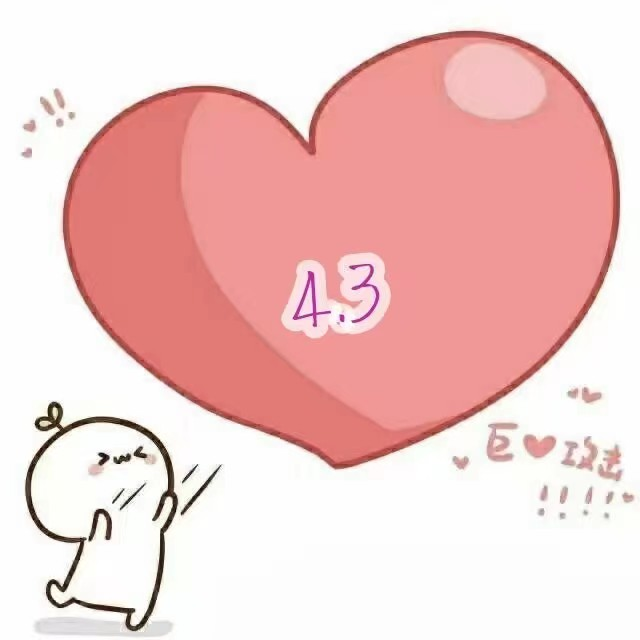
\includegraphics[width=\textwidth]{figs/4.3.jpg}
\end{figure}

\thispagestyle{empty}

\clearpage

\begin{center}
    \tableofcontents
\end{center}

\thispagestyle{empty}

\clearpage
\part{3.6 - 3.12}

\section*{P10-1.2.2.}

令$G$是实数对$(a,b)$, $a\ne 0$的集合. 在$G$上定义
$(a,b)(c,d)=(ac,ad+b)$. 试证$G$是群. 

\begin{proof}
当$a,c\ne 0$时$ac\ne 0$, 故$(a,b)(c,d)=(ac,ad+b)\in G$. 

结合律: 
\begin{gather*}
(a,b)(c,d)\cdot(e,f)=(ac,ad+b)(e,f)=(ace,acf+ad+b)\\
(a,b)\cdot(c,d)(e,f)=(a,b)(ce,cf+d)=(ace,acf+ad+b)
\end{gather*}

幺元: 
容易验证$(a,b)(1,0)=(1,0)(a,b)=(a,b)$. 

逆元: 
若$(a,b)\cdot(c,d)=(ac,ad+b)=(1,0)$, 则$(c,d)=(1/a,-b/a)$, 
此时也可验证$(1/a,-b/a)\cdot(a,b)=(1,0)$. 故$(a,b)^{-1}=(1/a,-b/a)$. 
\end{proof}

\section*{P10-1.2.6.\xuan}

设$G$是一个半群. 如果$G$中含有左幺元$e$, 即对任意$a\in G$有$ea=a$; 
且$G$的每个元素$a$都有左逆$a^{-1}$, 使得$a^{-1}a=e$. 试证$G$是群. 

\begin{proof}
任意$a\in G$有左逆$a^{-1}$, $a^{-1}$有左逆$(a^{-1})^{-1}$. 
由$aa^{-1}=eaa^{-1}=(a^{-1})^{-1}a^{-1}aa^{-1}=(a^{-1})^{-1}a^{-1}=e$
和$ae=aa^{-1}a=ea=a$, 得$e$是幺元, $a^{-1}$是$a$的逆元. 
因此$G$是群. 
\end{proof}

\section*{P11-1.2.9.}

设$G$是含幺半群, $a,b\in G$. 求证: 
如果$a$有逆元素$a^{-1}$, 则$a^{-1}$也有逆元素, 且$(a^{-1})^{-1}=a$; 
如果$a,b$都具有逆元素, 则$ab$也有逆元素, 且$(ab)^{-1}=b^{-1}a^{-1}$. 

\begin{proof}
如图. 

\begin{figure}[!htbp]
\centering
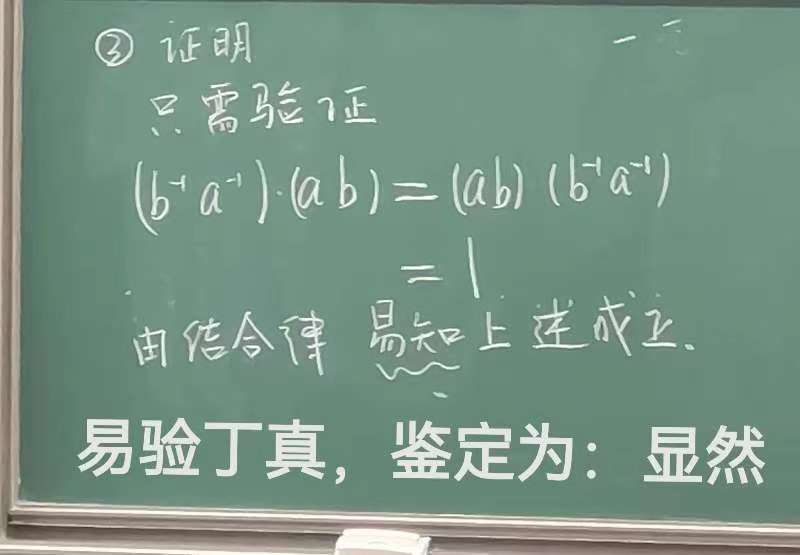
\includegraphics[width=.4\textwidth]{figs/yydz.jpg}
\end{figure}

\end{proof}

\section*{1.阅读}

设$A_i,i\in I$是一族非空集合, 定义这些集合的乘积
$\prod_{i\in I}A_i=\{(a_i)_{i\in I}:a_i\in A\}$, 
那么选择公理等价于$\prod_{i\in I}A_i\ne\emptyset$. 

\section*{2.}

考虑$\Z$的模$n$同余等价类集合$\Z_n=\Z/\sim\ =\{\cl{0},\cl{1},\cdots,\cl{n-1}\}$, 
在上面定义乘法$\cl{i}\cdot\cl{j}=\cl{ij}$. 

\subsection*{(1)}

请验证该运算是良定的. 

\begin{proof}
设$\cl{i}=\cl{i'}$, $\cl{j}=\cl{j'}$, 则存在$k_1,k_2\in\Z$
使得$i-i'=k_1n$, $j-j'=k_2n$. 故由
\[ij-i'j'=(i-i')j+i'(j-j')=k_1nj+k_2ni\equiv 0\mod{n}\]
得该运算良定. 
\end{proof}

\subsection*{(2)}

设$(\Z_n)^*=\{\cl{i}:\gcd(i,n)=1\}$, 
证明$(\Z_n)^*$在上述乘法下是一个群. 

\begin{proof}
设$\cl{a},\cl{b}\in(\Z_n)^*$, 则由$\gcd(a,n)=\gcd(b,n)=1$
得$\gcd(ab,n)=1$, 故$\cl{a}\cdot\cl{b}=\cl{ab}\in(\Z_n)^*$. 

结合律: 
由整数乘法结合律即得. 

单位元: 
容易验证$\cl{1}\cdot\cl{a}=\cl{a}\cdot\cl{1}=\cl{a}$. 

逆元: 
$\gcd(a,n)=1$, 由Bezout等式, 存在$s,t\in\Z$使得$as+nt=1$, 
故$as\equiv 1\mod{n}$, 且可得$\gcd(s,n)=1$, 故$\cl{s}\in(\Z_n)^*$. 
\end{proof}

\subsection*{(3)}

记$\varphi(n)=\abs{(\Z_n)^*}$, 称之为{\bf 欧拉函数}. 
设$p$是素数, $m$是正整数, 计算$\varphi(p^m)$, $\varphi(300)$. 

\begin{solution}
小于$p^m$且不与$p^m$互素的自然数只有$0,p,2p,\cdots,(p^{m-1}-1)p$, 
故$\varphi(p^m)=p^m-p^{m-1}$. 

由$\varphi$是积性的, 得$\varphi(300)=\varphi(2^2)\cdot\varphi(3)\cdot\varphi(5^2)
=2\cdot 2\cdot 20=80$. 
\end{solution}

\section*{3.}

记$\GL_n(\Z)$为行列式为$\pm 1$的整系数$n$阶方阵集合. 
验证$\GL_n(\Z)$关于矩阵乘法是一个群. 

\begin{proof}
设$A,B\in\GL_n(\Z)$, 则$\det(AB)=\det A\cdot\det B=\pm 1$.

结合律: 
矩阵乘法有结合律. 

单位元: 
容易验证$I_n\cdot A=A\cdot I_n=A$. 

逆元: 
对任意$A\in\GL_n(\Z)$, 可得$AA^*=A^*A=\det A\cdot I_n$, 
其中$A^*$为$A$的伴随矩阵. 由伴随矩阵定义和整数乘法封闭性可得
$A^*$为整数矩阵. 令$B=A^*/\det A$, 由于$\det A=\pm 1$, 
故$B$也是整数矩阵, 且$AB=BA=I_n$, $\det B=1/\det A=\pm 1$, 
因此$A$有逆元$B\in\GL_n(\Z)$. 
\end{proof}

\begin{remark}
这里有些群友直接由$\det A\ne 0$就得出$A$可逆, 
但这样不能保证$A^{-1}\in\GL_n(\Z)$, 
也就是说不能保证$A$的逆也是整数矩阵. 
\end{remark}

\section*{4.}

设$a$是群$G$中的元素, 约定$a^0=1$. 

\subsection*{(1)}

对于自然数$n$, 证明$(a^n)^{-1}=(a^{-1})^n$. 
后面约定$a^{-n}=(a^{-1})^n$. 

\begin{proof}
只要证$a^n(a^{-1})^n=(a^{-1})^na^n=1$. 这由结合律显然. 
\end{proof}

\subsection*{(2)}

设$k,l\in\Z$, 证明$a^{k+l}=a^k\cdot a^l$. 

\begin{proof}
$k,l\in\N$时由结合律显然. 

$k,l$有一个小于$0$时, 不妨设$k<0$. 若$k+l\ge 0$, 则
$a^{k+l}=1\cdot a^{k+l}=a^{k}\cdot a^{-k}a^{k+l}=a^ka^l$; 
若$k+l<0$, 则$a^{k+l}=(a^{-1})^{-k-l}=(a^{-1})^{-k-l}\cdot 1
=(a^{-1})^{-k-l}(a^{-1})^la^l=(a^{-1})^{-k}a^l=a^ka^l$. 

$k,l<0$时$a^{k+l}=(a^{-1})^{-k-l}=(a^{-1})^{-k}(a^{-1})^{-l}=a^ka^l$. 
\end{proof}

\clearpage
\part{3.13 - 3.19}

\section*{P11-1.2.15.}

对任意$a\in G$, $a\mapsto a^{-1}$是群$G$的自同构当且仅当$G$是交换群. 

\begin{proof}
令$f:G\to G,a\mapsto a^{-1}$.

$\implies$: 
对任意$a,b\in G$, 若$f\in\Aut G$, 则$ab=f(b^{-1}a^{-1})=f(b^{-1})f(a^{-1})=ba$. 

$\impliedby$: 
容易验证$f$是双射. 对任意$a,b\in G$, 有$f(a)f(b)=a^{-1}b^{-1}=(ba)^{-1}=f(ba)=f(ab)$. 
\end{proof}

\section*{P17-1.3.1.}

试证群$G$的任意多个子群的交仍是$G$的子群. 

\begin{proof}
设$A_i\le G$, $i\in I$. 对任意$a,b\in\bigcap_{i\in I}A_i$, 
由每个$A_i\le G$, 得$ab^{-1}\in A_i,\forall i\in I$. 
故$ab^{-1}\in\bigcap_{i\in I}A_i$, 
由\myref[subgroup]{\bf 1.3.2.}得$\bigcap_{i\in I}A_i\le G$. 
\end{proof}

\begin{remark}
这里$\bigcap_{i\in I}A_i$不能写成$\bigcap^\infty_{i=1}A_i$, 
更不能写成$\bigcap^n_{i=1}A_i$. 前者意味着可数, 后者意味着有限. 
\end{remark}

\section*{P17-1.3.2.}
\label{subgroup}

设$A$是群$G$的非空子集. 试证$A$是$G$的子群当且仅当对任意
$a,b\in A$有$ab^{-1}\in A$\kh{这也相当于$AA^{-1}=A$}. 

\begin{proof}
$\implies$: 
若$A\le G$, 则对任意$a,b\in A$有$b^{-1}\in A$, 进而有$ab^{-1}\in A$. 

$\impliedby$: 
结合律显然. 
幺元: 对任意$a\in A$, 有$aa^{-1}=1\in A$. 
逆元: 令$a=1$, 则对任意$b\in A$有$b^{-1}\in A$. 
封闭性: 对任意$a,b\in A$, 可知$b^{-1}\in A$, 
故$a(b^{-1})^{-1}=ab\in A$. 
\end{proof}

\section*{P17-1.3.5.\normalsize 重要}

设$A,B$是群$G$的两个子群. 试证: $AB$是$G$的子群当且仅当$AB=BA$. 

\begin{proof}
$\implies$: 对任意$a\in A,b\in B$有$ab\in AB$. 对任意$a\in A,b\in B$, 
由$A,B\le G$有$a^{-1}\in A,b^{-1}\in B$. 对任意$ba\in BA$, 
注意到$ba=(a^{-1}b^{-1})^{-1}$和$a^{-1}b^{-1}\in AB$, 
又由$AB\le G$有$(a^{-1}b^{-1})^{-1}=ba\in AB$, 得$BA\subseteq AB$. 

另一方面, 对任意$ab\in AB$, 由$AB\le G$可知$b^{-1}a^{-1}=
(ab)^{-1}\in AB$, 故存在$a'\in A,b'\in B$使得$b^{-1}a^{-1}=a'b'$. 
同时由$a^{-1}\in A,b^{-1}\in B$可得$a'b'=b^{-1}a^{-1}\in BA$,
故$ab=(b^{-1}a^{-1})^{-1}=b'^{-1}a'^{-1}\in BA$, 得$AB\subseteq BA$. 
因此有$AB=BA$. 

$\impliedby$: 对任意$a_1b_1,a_2b_2\in AB$, 其中$a_1,a_2\in A$, $b_1,b_2\in B$, 
有$a_1b_1(a_2b_2)^{-1}=a_1b_1b_2^{-1}a_2^{-1}\in ABA=AAB=AB$, 
故由\myref[subgroup]{\bf 1.3.2.}得$AB\le G$. 
\end{proof}

\begin{remark}
这里我看到有几位群友证得$BA\subseteq AB$后构造了个双射$f:AB\to BA$
或$g:BA\to AB$, 试图以此证明$BA=AB$. 然而对于集合$S_2\subseteq S_1$, 
即使存在双射$f:S_1\to S_2$, 也未必有$S_1=S_2$. 一个反例是$S_1=\Z\supsetneq 2\Z=S_2$, 
可知$f:S_1\to S_2$, $n\mapsto 2n$为双射. 但是如果$S_1\subseteq S_2$是有限集, 
且存在双射$f:S_1\to S_2$, 那么一定有$S_1=S_2$. 
\end{remark}

\section*{P18-1.3.13.}

设$a,b$是群$G$的任意两个元素. 试证: $a$和$a^{-1}$, $ab$和$ba$有相同的阶. 

\begin{proof}
若$\ord(a)<\infty$, 设$\ord(a)=m$. 由$a^m=1$得$(a^{-1})^m=(a^m)^{-1}=1$, 
可知$\ord(a^{-1})\mid m$, 同理$m\mid\ord(a^{-1})$, 
故$\ord(a)=\ord(a^{-1})$. 

若$\ord(a)=\infty$, 假设$\ord(a^{-1})=m'<\infty$, 
则$(a^{m'})^{-1}=(a^{-1})^{m'}=1$, 即$a^{m'}=1$, 矛盾, 得$\ord(a^{-1})=\infty$. 

\vspace{1em}

若$\ord(ab)<\infty$, 设$\ord(ab)=m$, 则由$(ba)^{m+1}=b(ab)^ma=ba$知$(ba)^m=1$, 
得$\ord(ba)\mid m$, 同理$m\mid\ord(a^{-1})$, 故$\ord(ab)=\ord(ba)$. 

若$\ord(ab)=\infty$, 假设$\ord(ba)=m'<\infty$, 
则$(ab)^{m'}=a(ba)^{m'}a^{-1}=a\cdot 1\cdot a^{-1}=1$, 矛盾, 得$\ord(ba)=\infty$. 
\end{proof}

\begin{remark}
这里有不少群友没考虑$\ord(a)=\infty$和$\ord(ab)=\infty$的情况. 
\end{remark}

\section*{1.}
\label{f-with-f(1)}

设$G$是一个群, 取$g\in G$, 则$g$决定了一个群同态
$f_g:\Z\to G$, $i\mapsto g^i$. 反过来, 一个群同态
$f:\Z\to G$由$f(1)$唯一确定. 

\begin{proof}
对任意$i,j\in\Z$,可知$f_g(i+j)=g^{i+j}=g^i\cdot g^j=f(i)\cdot f(j)$, 
故$f_g:\Z\to G$为群同态. 

反过来, 对每个群同态$f:\Z\to G$和任意的$i\in\N$, 
有$f(i)=f(\overbrace{1+\cdots+1}^i)=f(1)^i$, 而$i\in\Z_{<0}$时
$f(i)=f(-i)^{-1}=f(\underbrace{1+\cdots+1}_{-i})^{-1}=f(1)^i$, 
故$f$可由$f(1)$唯一确定. 
\end{proof}

\section*{2.}

利用{\bf 1.}所述结论确定$\Aut(\Z,+)$, 以及用这种思想确定$\Aut(\Q,+)$. 

\begin{solution}
对$f\in\Aut(\Z,+)$, 设$f(1)=a$, 故对任意$b\in\Z$, 有$f(b)=f(1)\cdot b=ab$, 
且$f$为满射, 即存在$b\in\Z$有$ab=1$, 因此$a=\pm 1$. 故$\Aut(\Z,+)=\{b\mapsto ab:a=\pm 1\}=(\Z/2\Z,+)$. 

对$g\in\Aut(\Q,+)$, 设$g(1)=a$, 故对任意$q\in\Z_{>0}$, 有$g(1)=f(\overbrace{1/q+...+1/q}^q)=g(1/q)\cdot a$, 
故$g(1/q)=a/q$. 对任意$p\in\Z$, 与上段类似地有$g(p/q)=g(1/q)\cdot p=ap/q$, 且$a\ne 0$时容易验证$g^{-1}(r)=r/a$. 
故$\Aut(\Q,+)=\{r\mapsto ar:a\in\Q^*\}\isom(\Q^*,\cdot)$. 
\end{solution}

\section*{3.}

在$S_3$中找一个子群$H$使得存在置换$\sigma$满足$\sigma H\ne H\sigma$. 

\begin{solution}
\kh{不唯一; 这个我懒得算了, 参考一下某位群友的作业} 
注意到$(12)(123)=(13)$, $(123)(12)=(23)$. 令$H=\{1,(12)\}$, 
$\sigma=(123)$, 则$\sigma H=\{(123),(23)\}\ne\{(123),(13)\}=H\sigma$. 
\end{solution}

\section*{4.}
\label{GL-SL}

考虑子群$\SL(n,\R)\le\GL(n,\R)$. 证明: 两个矩阵属于
$\SL(n,\R)$的同一个左陪集当且仅当它们的行列式相等. 

\begin{proof}
$\implies$: 
设$A,B\in\GL(n,\R)$属于$\SL(n,\R)$的同一个左陪集$A\cdot\SL(n,\R)$, 
则存在$C\in\SL(n,\R)$使得$B=AC$, 故$\det B=\det A\cdot\det C=\det A\cdot 1=\det A$. 

$\impliedby$: 
设$A,B\in\GL(n,\R)$满足$\det A=\det B\ne 0$, 则有$\det A^{-1}B=\det A^{-1}\cdot\det B=1$, 
即$A^{-1}B\in\SL(n,\R)$, 故$B=AA^{-1}B\in A\cdot\SL(n,\R)$, 
即$A,B$属于$\SL(n,\R)$的同一个左陪集. 

令$\F$为$\SL(n,\R)$的所有左陪集, $f:\mathcal{F}\to\R^*,A\cdot\SL(n,\R)\mapsto\det A$. 
由上述证明可知$f$是良定的, 且为$\mathcal{F}$与$\R^*$之间的双射. 
\end{proof}

\section*{5.\normalsize 重要}

设群$G$中的元素$a,b$的阶分别为$m,n$, 如果$ab=ba$
且$\gcd(m,n)=1$. 

\subsection*{(1)}

证明对任意$i,j\in\Z$有$a^ib^j=b^ja^i$\kh{因为非常显然, 不怀疑的话不用证}. 

\begin{proof}
不妨设$0\le i\le m-1$, $0\le j\le n-1$, 这样就显然了. 
\end{proof}

\subsection*{(2)}

课上已经证明过$\gen{a}=\{1,a,\cdots,a^{m-1}\}$是$G$的子群, 
请证明$\gen{a}\cap\gen{b}=\{1\}$. 

\begin{proof}
若$\gen{a}\cap\gen{b}\ne\{1\}$, 
由$\gen{a}\cap\gen{b}\le\gen{a}$
也是循环群, 得$\gen{a}\cap\gen{b}$有生成元$c\ne 1$. 
设$\ord(c)=u>1$, 则可知$u\mid m$, $u\mid n$, 这与$\gcd(m,n)=1$矛盾. 
\end{proof}

\subsection*{(3)}
\label{ord-mul}

$\ord(ab)=mn$. 

\begin{proof}
对任意的$s\in\{1,...,m-1\}$, $t\in\{1,...,n-1\}$, 假如$a^sb^t=1$, 
则$a^s=b^{-t}=b^{n-t}$, 且$n-t\in\{1,...,n-1\}$, 由(2)得此时只能有$a^s=b^{n-t}=1$, 
这与$\ord(a)=m$, $\ord(b)=n$矛盾, 故总有$a^sb^t\ne 1$, 进而可以得到
$a^sb^t=1$当且仅当$m\mid s$, $n\mid t$. 对$d\in\Z$, 若$(ab)^d=a^db^d=1$, 
则有$m\mid d$, $n\mid d$, 故$mn=\lcm(m,n)\mid d$. 又$(ab)^{mn}=a^{mn}b^{mn}=1$, 得$\ord(ab)=mn$. 
\end{proof}

\section*{6.\normalsize 如果觉得显然就阅读}

设$A,B,C$是群$G$的非空子集, 定义
$A\cdot B=\{a\cdot b:a\in A,\ b\in B\}$和
$A^{-1}=\{a^{-1}:a\in A\}$. 
验证: $(AB)C=A(BC)$, $(AB)^{-1}=B^{-1}A^{-1}$, 
$gA=gB\iff A=B$, 以及$gA=B\iff A=g^{-1}B$. 

\begin{proof}
直接按定义验证即可. 
\end{proof}

\section*{7.}

设$A\le G$, 证明作为集合有$(gA)^{-1}=Ag^{-1}$, 
以此可以直接证明左右陪集一一对应. 

\begin{proof}
\kh{这个上课是不是也证过}一方面, 对任意$x=(ga)^{-1}\in(gA)^{-1}$, 
由$x=a^{-1}g^{-1}$和$a^{-1}\in A$得$x\in Ag^{-1}$, 故$(gA)^{-1}\subseteq Ag^{-1}$; 
另一方面, 对任意$y=ag^{-1}\in Ag^{-1}$, 由$x=(ga^{-1})^{-1}$和
$a^{-1}\in A$得$x\in(gA)^{-1}$, 故$Ag^{-1}\subseteq(gA)^{-1}$. 
因此$(gA)^{-1}=Ag^{-1}$. 
\end{proof}

\section*{8.\xuan}

设$G$为有限群, $A,B$为$G$的子群, 课上已经证明了$C=A\cap B$
也是子群, 设$[A:C]=k$, 记$\{a_1C,\cdots,a_kC\}$为$C$在$A$
中的所有左陪集. 请证明: 

\subsection*{(1)}

对于$i\ne j$, 左陪集$a_iB\ne a_jB$. 

\begin{proof}
对于$i\ne j$, 可知$a_iC\ne a_jC$, 即$a_i^{-1}a_j\notin C=A\cap B$. 
由$a_i,a_j\in A\le G$得$a_i^{-1}a_j\in A$, 故$a_i^{-1}a_j\notin B$, 
即$a_iB\ne a_jB$. 
\end{proof}

\subsection*{(2)}

对于任意$a\in A$, 存在$i\in\{1,2,\cdots,k\}$使得$aB=a_iB$. 

\begin{proof}
对于任意$a\in A$, 由于$C\le A$且$C$在$A$中的所有左陪集为$a_1C,...,a_kC$, 
得存在$i$有$aC=a_iC$, 故$a^{-1}a_i\in C\le B$, 得$aB=a_iB$. 
\end{proof}

\subsection*{(3)}

由{\bf (1)(2)}可得$A\cdot B=\bigsqcup^k_{i=1}a_iB$, 
从而$\abs{A\cdot B}=\abs{A}\cdot\abs{B}/\abs{A\cap B}$. 

\begin{proof}
由{\bf (1)(2)}可得$A\cdot B=\bigsqcup^k_{i=1}a_iB$, 故$\abs{AB}=k\cdot\abs{B}=\abs{B}\cdot\abs{A}/\abs{A\cap B}$. 
\end{proof}

\subsection*{(4)}

用类似的办法处理{\bf P18-1.3.11.}: 设$H$和$K$分别是有限群$G$的两个子群, 
试证$\abs{HgK}=\abs{H}\cdot[K:g^{-1}Hg\cap K]$. 

\begin{proof}
容易验证$\abs{HgK}=\abs{g^{-1}HgK}$, $g^{-1}Hg\le G$且$\abs{g^{-1}Hg}=\abs{H}$. 
因此\[\abs{HgK}=\abs{g^{-1}HgK}=\frac{\abs{g^{-1}Hg}\cdot\abs{K}}{\abs{g^{-1}Hg\cap K}}=\abs{H}\cdot[K:g^{-1}Hg\cap K].\]
\end{proof}

\begin{remark}
这里我看到有几位群友对$H$和$gK$应用{\bf (3)}的结论得出
$\abs{HgK}=\abs{H}\cdot\abs{gK}/\abs{H\cap gK}$, 
但$gK$未必是$G$的子群, 所以不能直接用{\bf (3)}. 
\end{remark}

\section*{9.}

设$G$是一个群, 满足对于所有的元素$a$有$a^2=1$. 
证明群$G$是交换群. 

\begin{proof}
可知对任意$a\in G$都有$a^{-1}=a$. 因此对任意$a,b\in G$有
$ab=(ab)^{-1}=b^{-1}a^{-1}=ba$, 故$G$为交换群. 
\end{proof}

\clearpage
\part{3.20 - 3.26}

\section*{P20-1.4.2.}

证明: 群$G$没有非平凡子群的充分必要条件是$G=\{1\}$
或$G$是素数阶循环群. 

\begin{proof}
$\implies$: 
首先$\{1\}$没有非平凡子群. 其次, 若$G\ne\{1\}$则存在$g\in G\setminus\{1\}$. 
当$\abs{G}=\infty$时, 若$\ord(g)<\infty$则$\gen{g}<G$, 若$\ord(g)=\infty$
则$\gen{g^2}<\gen{g}\le G$, 矛盾. 当$\abs{G}<\infty$时对每个$g\in G\setminus\{1\}$
都有$\gen{g}=G$, 得$G$为循环群. 假设$\abs{G}=ab$为合数 (其中$a,b\in\N_+$), 
则由$(g^a)^b=1$可知$\gen{g^a}<G$, 矛盾, 故只能有$G$为素数阶循环群. 

$\impliedby$: 
$\{1\}$没有非平凡子群. 假设素数$p$阶循环群$G$有子群$H\le G$, 
则由$\abs{H}\mid p=\abs{G}$得$\abs{H}=1$或$p$, 都是$G$的平凡子群. 
\end{proof}

\section*{P20-1.4.4.}

设$a$和$b$是群$G$的元素, 阶数分别是$n$和$m$, 
$\gcd(n,m)=1$且$ab=ba$. 试证$\gen{ab}$是$G$的$mn$阶循环子群. 

\begin{proof}
同\myref[ord-mul]{\bf 第2周5.(3)}. 
\end{proof}

\section*{P20-1.4.6.}

设$G$是一个$n$阶有限群, 若对$n$的每一因子$m$, 
$G$中至多只有一个$m$阶子群, 则$G$是循环群. 

\begin{proof}
先证明对$n$的每个正因子$m$, $G$中阶为$m$的元素至多有$\varphi(m)$个. 
假如有超过$\varphi(m)$个, 设其中一个为$a$, 则$\gen{a}<G$, 
$\gen{a}$中阶为$m$的元素有$\varphi(m)$个, 故存在阶为$m$的$b\in G\setminus\gen{a}$, 
得$G$有至少两个$m$阶子群$\gen{a},\gen{b}$, 矛盾. 

设$G$中阶为$m$的元素有$f(m)$个, 则$f(m)\le\varphi(m)$. 由
$n=\sum_{m\mid n}f(m)\le\sum_{m\mid n}\varphi(m)=n$
得$f(m)=\varphi(m)$, 特别地有$f(n)=\varphi(n)\ge 1$, 
即$G$中存在$n$阶元, 故为循环群. 
\end{proof}

\begin{remark}
可以用这个命题证明有限域的单位群$(\F_{p^n})^*$为循环群. 
\end{remark}

\section*{P25-1.5.2.}

设$G$是群, $N<M<G$. 

\subsection*{(1)}

如果$N\lhd G$, 则$N\lhd M$. 

\begin{proof}
由$N\lhd G$, 得对任意$g\in G$有$gNg^{-1}=N$, 
故对任意$g\in M<G$有$gNg^{-1}=N$, 又$N<M$, 得$N\lhd M$. 
\end{proof}

\subsection*{(2)}

如果$N\lhd M$, 那$N$是否一定是$G$的正规子群? 

\begin{solution}
不一定. 以下给出群友们的智慧: 

\begin{itemize}[itemsep=0em]
    \item $\Z_2\lhd K_4\lhd A_4$, 但$\Z_2\nlhd A_4$. 
    \item $N$为所有对角元为$1$的$n$阶上三角实方阵, $M$为所有对角元非零的$n$阶上三角实方阵, $G=\text{GL}_n(\R)$, 则$N\lhd M<G$, 但$N\nlhd G$. 
    \item 自由群$\gen{a^2}\lhd\gen{a}<\gen{a,b}$, 但$\gen{a^2}\nlhd\gen{a,b}$. 
\end{itemize}
\end{solution}

\section*{P25-1.5.4.}

试证群$G$的指数为$2$的子群一定是$G$的正规子群. 

\begin{proof}
设$H\lhd G$, $[G:H]=2$. 对任意$g\in G\setminus H$, 则$G=H\sqcup gH=H\sqcup Hg$, 
故$gH=Hg=G\setminus H$, 即$gHg^{-1}=H$; 而对任意$g\in H$有$gH=Hg=H$, 也有$gHg^{-1}=H$. 
因此$H\lhd G$. 
\end{proof}

\section*{P25-1.5.7.}

设$M$和$N$分别是群$G$的正规子群. 如果$M\cap N=\{1\}$, 
则对任意$a\in M$, $b\in N$, 都有$ab=ba$. 

\begin{proof}
只要证$ab(ba)^{-1}=aba^{-1}b^{-1}=1$. 注意到$aba^{-1}\in aNa^{-1}=N$
且$b^{-1}\in N$, 有$aba^{-1}\cdot b^{-1}\in N$; 又$ba^{-1}b^{-1}\in bMb^{-1}=M$
且$a\in M$, 有$a\cdot ba^{-1}b^{-1}\in M$, 故$aba^{-1}b^{-1}\in M\cap N=\{1\}$. 
\end{proof}

\section*{1.}

设$G$是有限群, 假设存在元素$a$使得$G=\gen{a}$, 
此时称$G$为{\bf 循环群}, $a$称作$G$的一个{\bf 生成元}. 

\subsection*{(1)}

群同态$f:G\to K$由$f(a)$唯一确定. 

\begin{proof}
与\myref[f-with-f(1)]{\bf 第2周1.}证明$f:\Z\to K$由$f(1)$唯一确定的思路类似. 
\end{proof}

\subsection*{(2)}

如果$f:\Z_{12}\to\Z_{16}$是一个群同态, 设$f(\cl{1})=\cl{k}\in\Z_{16}$, 
问$\cl{k}$可以取哪些值? 

\begin{solution}
群同态$f:\Z_{12}\to\Z_{16}$由$f(\cl{1})=\cl{k}$唯一确定, 由$12\cdot\cl{k}=f(12\cdot\cl{1})=f(\cl{0})=\cl{0}$
得$\ord(\cl{k})\mid 12$, 又$\ord(\cl{k})\mid 16$, 得$\ord(\cl{k})\mid\gcd(12,16)=4$, 
故$\cl{k}\in\{\cl{0},\cl{4},\cl{8},\cl{12}\}$. 
\end{solution}

\section*{2.\xuan}

证明: $\Aut\Z_n\isom(\Z_n)^*$\kh{注意证明群同构, 不仅仅一一对应}. 

\begin{proof}
$f\in\Aut\Z_n$由$f(\cl{1})$唯一确定, 记$f_{\cl{a}}$为满足$f(\cl{1})=\cl{a}$的自同构$f$. 

由于$f_{\cl{a}}$为自同构, 故$\ord(\cl{a})=\ord(\cl{1})=n$. 设$\gcd(n,a)=d$, 
则由$n\mid n/d\cdot a$得$n/d\cdot\cl{a}=\cl{0}$, 故$\ord(\cl{a})\mid n/d$, 
因此有$d=1$, 即$\cl{a}\in(\Z_n)^*$. 反过来, 每个$\cl{a}\in(\Z_n)^*$
决定一个$f_{\cl{a}}:\cl{1}\mapsto\cl{a}$. 

令$g:(\Z_n)^*\to\Aut\Z_n,\cl{a}\mapsto f_{\cl{a}}$, 则$g$为双射. 
注意到$f_{\cl{a}}\circ f_{\cl{b}}(1)=f_{\cl{a}}(\cl{b})=\cl{b}\cdot f_{\cl{a}}(\cl{1})=\cl{b}\cdot\cl{a}=\cl{ab}$, 
可得$f_{\cl{a}}\circ f_{\cl{b}}=f_{\cl{ab}}$, 即$g(a)g(b)=g(ab)$, 得$g$为同构. 
\end{proof}

\section*{3.}

证明: $\gen{\cl{22},\cl{55}}=\Z_{100}$. 

\begin{proof}
显然$\gen{\cl{22},\cl{55}}\le\Z_{100}$. 由$\cl{11}=\cl{55}-2\cdot\cl{22}$
和$\gcd(11,100)=1$, 得$\cl{11}$是$\Z_{100}$的生成元, 
故$\gen{\cl{22},\cl{55}}\ge\gen{\cl{11}}=\Z_{100}$. 
因此有$\gen{\cl{22},\cl{55}}=\Z_{100}$. 
\end{proof}

\section*{4.}

设$N$是$G$的正规子群, 验证$aN\cdot bN=abN$\kh{集合乘积}. 

\begin{proof}
由$N\lhd G$得$bN=Nb$, 故$aN\cdot bN=a\cdot Nb\cdot N=a\cdot bN\cdot N=abN$. 
\end{proof}

\section*{5.}

描述$\Z_{12}$到$\Z_{20}$的所有群同态. 

\begin{solution}
群同态$f:\Z_{12}\to\Z_{20}$由$f(\cl{1})=\cl{k}$唯一确定, 
由$12\cdot\cl{k}=f(12\cdot\cl{1})=f(\cl{0})=\cl{0}$得$\ord(\cl{k})\mid 12$, 
又$\ord(\cl{k})\mid 20$, 得$\ord(\cl{k})\mid\gcd(12,20)=4$, 
故$\cl{k}\in\{\cl{0},\cl{5},\cl{10},\cl{15}\}$, 
即$\Z_{12}$到$\Z_{20}$的所有群同态为$\{f_{\cl{0}},f_{\cl{5}},f_{\cl{10}},f_{\cl{15}}\}$. 
\end{solution}

\section*{6.}

设$A$是群$G$的非空子集. 

\subsection*{(1)}

证明集合$N_G(A)=\{g\in G:g^{-1}Ag=A\}$是一个子群, 称作$A$的{\bf 正规化子群}. 

\begin{proof}
$1\in N_G(A)\ne\emptyset$. 对任意$g,h\in N_G(A)$, 有
$g^{-1}hAh^{-1}g=g^{-1}h\cdot h^{-1}Ah\cdot h^{-1}g=g^{-1}Ag=A$, 
故$gh^{-1}\in N_G(A)$, 得$N_G(A)\le G$. 
\end{proof}

\subsection*{(2)}

证明集合$C_G(A)=\{g\in G:ga=ag,\forall a\in A\}$是一个子群, 
称作$A$的{\bf 中心化子群}. 

\begin{proof}
$1\in C_G(A)\ne\emptyset$. 由$ga=ag$得$g^{-1}ag=gag^{-1}=a$. 
对任意$g,h\in C_G(A)$, 有$gh^{-1}ahg^{-1}=gag^{-1}=a$, 
即$gh^{-1}a=agh^{-1}$, 故$gh^{-1}\in C_G(A)$, 得$C_G(A)\le G$. 
\end{proof}

\subsection*{(3)}

当$A=G$时, 子群$C_G(G)$通常记作$C(G)$, 称作$G$的{\bf 中心}, 
证明$C(G)$是$G$的正规子群. 

\begin{proof}
对任意$x\in C(G)$和任意$g\in G$有$gxg^{-1}=x$, 
故$gC(G)g^{-1}=\{gxg^{-1}:x\in C(G)\}=C(G)$, 
得$C(G)\lhd G$. 
\end{proof}

\subsection*{(4)\xuan}

证明: 如果$G/C(G)$是循环群, 那么$G$是交换群. 

\begin{proof}
设$G/C(G)=\gen{a}$, 则对任意$g,h\in G$, 
存在$x,y\in C(G)$和$m,n\in\Z$有$g=a^mx,h=a^ny$. 
因此有$gh=a^mxa^ny=a^ma^nxy=a^na^myx=a^nya^mx=hg$, 
得$G$为交换群. 
\end{proof}

\section*{7.}

证明群同构$\GL_n(\R)/\SL_n(\R)\isom\R^*$. 

\begin{proof}
设$f:\GL_n(\R)\to\R^*$, $A\mapsto\det A$. 
由$f(AB)=\det AB=\det A\cdot\det B=f(A)f(B)$得$f$为群同态. 
对任意$a\in\R^*$, 由$f(\mathrm{diag}(a,1,...,1))=a$, 得$\im f=\R^*$. 
又$\ker f=f^{-1}(1)=\SL_n(\R)$, 故由同态基本定理得
$\GL_n(\R)/\SL_n(\R)\isom\im f=\R^*$. 
\end{proof}

布置这个题的时候还没学同态基本定理, 这里再给出一种直接把陪集映射到行列式的做法. 

\begin{proof}
设$g:\GL_n(\R)/\SL_n(\R)\to\R^*$, $\cl{A}=A\cdot\SL_n(\R)\mapsto\det A$. 
\myref[GL-SL]{\bf 第2周4.}已证得$g$为良定的双射. 又$g(\cl{A})\cdot g(\cl{B})=
\det A\cdot\det B=\det AB=g(\cl{AB})$, 得$g$为同构. 
\end{proof}

\clearpage
\part{3.27 - 4.2}

\section*{P25-1.5.6.}

设$f:G\to H$是群同态, $M\le G$, 试证$f^{-1}(f(M))=KM$, 这里$K=\ker f$. 

\begin{proof}
对任意$x\in f^{-1}(f(M))$, 有$f(x)\in f(M)$, 故存在$m\in M$有
$f(x)=f(m)$. 因此有$f(xm^{-1})=f(x)\cdot f(m)^{-1}=1$, 得$xm^{-1}\in\ker f=K$, 
故$x=xm^{-1}\cdot m\in KM$. 因此$f^{-1}(f(M))\subseteq KM$. 
对任意$x\in KM$, 存在$k\in K$和$m\in M$有$x=km$, 故
$f(x)=f(k)f(m)=f(m)\in f(M)$. 因此$f^{-1}(f(M))\supseteq KM$. 
综上, 有$f^{-1}(f(M))=KM$. 
\end{proof}

\begin{remark}
这里有的群友试图通过证明$f(M)=f(KM)$来证得结论, 但这与待证命题不等价. 
容易注意到$f(M)=f(M)$, 但$K$不是$M$的子群时$f^{-1}(f(M))\ne M$. 
$f^{-1}(f(M))$是集合$f(M)$中元素\yh{所有}原像组成的集合, 要证明的是
\yh{所有}原像正好是集合$KM$. 
\end{remark}

\section*{P25-1.5.8.}

设$f:G\to H$是群同态. 如果$g$是$G$的一个有限阶元素, 则$f(g)$的阶整除$g$的阶. 

\begin{proof}
设$\ord(g)=n$, 则$g(n)=1$, 故$f(g)^n=f(g^n)=f(1)=1$, 得$\ord(f(g))\mid n=\ord(g)$. 
\end{proof}

\section*{P25-1.5.9.}

设$N\lhd G$, $g$是群$G$的任意一个元素. 如果$g$的阶和$\abs{G/N}$
互素, 则$g\in N$. 

\begin{proof}
设$\ord(g)=n$, 则$\cl{g}^n=\cl{g^n}=\cl{1}$, 
得$\ord(\cl{g})\mid n$. 又$\abs{G/N}<\infty$, 得
$\ord(\cl{g})\mid\abs{G/N}$. 因此$\ord(\cl{g})\mid\gcd(n,\abs{G/N})=1$, 
得$\cl{g}=\cl{1}$, 即$g\in N$. 
\end{proof}

\section*{P30-1.6.1.}

把置换$\sigma=(456)(567)(761)$写成不相交轮换的积. 

\begin{solution}
\sout{偷懒}方便起见, $2$和$3$省略. 
\[(1,4,5,6,7)\rto{(761)}(7,4,5,1,6)\rto{(567)}(5,4,6,1,7)\rto{(456)}(6,5,4,1,7)\]
可见$\sigma=(16)(45)$. 
\end{solution}

\section*{P30-1.6.2.}

讨论置换$\sigma=\pmat{1&2&\cdots&n\\n&n-1&\cdots&1}$的奇偶性. 

\begin{solution}
注意到$\sigma=(1n)(2,n-1)\cdots(\floor{n/2},n+1-\floor{n/2})$, 
为$\floor{n/2}$个对换之积, 
故$\sigma$的奇偶性与$\floor{n/2}$奇偶性相同, 
即$n\equiv 0,1\mod{4}$时$\sigma$为奇置换, 
$n\equiv 2,3\mod{4}$时$\sigma$为偶置换. 
\end{solution}

\begin{remark}
如果还记得线性代数讲行列式时讲过的\yh{逆序数}, 
可以发现$\sigma$的每一对都是逆序对, $\sigma$的逆序数为
$\mathrm{C}^2_n=\frac12n(n-1)$, 故$\sigma$的奇偶性与
$\frac12n(n-1)$的奇偶性相同, 即$n\equiv 0,1\mod{4}$时
$\sigma$为奇置换, $n\equiv 2,3\mod{4}$时$\sigma$为偶置换. 
\end{remark}

\section*{P30-1.6.4.}

设$\sigma=(12\cdots n)$为$S_n$的一个全轮换, 
试证$C_{S_n}(\sigma)=\gen{\sigma}$. 

\begin{proof}
对任意$\tau\in\gen{\sigma}$, 设$\tau=\sigma^i$, 
则$\tau\sigma=\sigma^{i+1}=\sigma\tau$, 
故$\gen{\sigma}\subseteq C_{S_n}(\sigma)$. 
对任意$\tau\in C_{S_n}(\sigma)$和任意$j\in\Z_n$, 
可知$\tau(j+1)=\tau\sigma(j)=\sigma\tau(j)
=\tau(j)+1\mod{n}$. 设$\tau(1)=k$, 则递推可知
$\tau(j)=k+j-1\mod{n}$, 得$\tau=\sigma^{k-1}\in\gen{\sigma}$. 
综上, 有$C_{S_n}(\sigma)=\gen{\sigma}$. 
\end{proof}

还有一位群友给出了这样的做法. 

\begin{proof}
对任意$\tau\in\gen{\sigma}$, 设$\tau=\sigma^i$, 
则$\tau\sigma=\sigma^{i+1}=\sigma\tau$, 
故$\gen{\sigma}\subseteq C_{S_n}(\sigma)$. 
$\sigma$所在的共轭类$C_\sigma$
为所有$n^1$型置换的集合, 故$\abs{C_\sigma}=(n-1)!$. 
由$\abs{C_\sigma}\cdot\abs{C_G(\sigma)}=\abs{S_n}=n!$, 
得$\abs{C_{S_n}(\sigma)}=n$. 又$\abs{\gen{\sigma}}=n$, 
$\gen{\sigma}\subseteq C_{S_n}(\sigma)$, 
得$C_{S_n}(\sigma)=\gen{\sigma}$. 
\end{proof}

\begin{remark}
对任意群$G$和$g\in G$, 有$\abs{C_g}=[G:C_G(g)]$. 证明在书上P16. {\rm\cite{jsds}}
\end{remark}

\section*{P30-1.6.5.}

试证一个置换的阶等于它的轮换表示中各个轮换的长度的最小公倍数. 

\begin{proof}
设$\sigma_1,\cdots,\sigma_k$为不相交轮换, 长度分别为$n_1,\cdots,n_k$, 
则易知$\ord(\sigma_i)=n_i$. 令$\tau=\sigma_1\cdots\sigma_k$. 
由于这些$\sigma_i$不相交, 可知其中任意两个可交换, 
故由$\tau^m=\sigma_1^m\cdots\sigma_k^m=1$得
对每个$i$都有$\sigma_i^m=1$, 故$n_i\mid m$, 
因此$\lcm(n_1,\cdots,n_k)\mid m$. 又$m=\lcm(n_1,\cdots,n_k)$
时即有$\tau^m=1$, 故$\ord(\tau)=\lcm(n_1,\cdots,n_k)$. 
\end{proof}

\section*{P30-1.6.6.}

试确定$S_4$的全部正规子群. 

\begin{solution}
$S_4$有两个平凡正规子群$\{1\}$和$S_4$. 可知$S_4$的非平凡正规子群$H$
是一些共轭类之并, 而且只可能是$2,3,4,6,8,12$阶. 先对$S_4$中的元素按
共轭类分类, 即按型分类: 
\begin{itemize}[itemsep=0pt]
    \item $1^1$型: $1$个
    \item $2^1$型: $\mathrm{C}^2_4=6$个
    \item $2^2$型: $\mathrm{C}^2_4/2=3$个
    \item $3^1$型: $\mathrm{C}^3_4\cdot(3-1)!=8$个
    \item $4^1$型: $(4-1)!=6$个
\end{itemize}

$S_4$的子群一定包含$1$, 因此只可能有$\abs{H}=4=1+3$
或$\abs{H}=12=1+3+8$. $\abs{H}=4$时$H$只包含$1$和
所有$2^2$型置换, 故$H=\{1,(12)(34),
(13)(24),(14)(23)\}$, 容易验证此时$H\isom K_4$; 
$\abs{H}=12$时$H$只包含$1$, 所有$2^2$型和所有$3^1$型置换, 
即包含所有偶置换, 此时$H=A_4$. 
因此$S_4$的所有正规子群有$\{1\},K_4,A_4,S_4$. 
\end{solution}

\begin{remark}
\myref[A4-lhd]{\bf 第4周习题课讲义1.}\yh{求$A_4$全部正规子群}的方法可以照葫芦画瓢
用在这个题上, 但上段所述方法用于求$A_4$正规子群时要谨慎. 对$A_n$中
的元素按共轭类分类时不能简单地按型分类, 
如$(123)$和$(132)$在$S_4$中是共轭的, 但在$A_4$中不是. 
\end{remark}

证明$(123),(132)\in A_4$不共轭: 

\begin{proof}
假设存在$\sigma\in A_4$
有$\sigma(123)\sigma^{-1}=(\sigma(1)\sigma(2)\sigma(3))=(132)=(321)=(213)$, 
可知$\{1,2,3\}$中必有一个是$\sigma$的不动点, 而另外两个被$\sigma$对换. 
比如设$1$为$\sigma$的不动点, 则$\sigma=(23)$. 这样的$\sigma$是奇置换, 
与$\sigma\in A_4$矛盾. 
\end{proof}

\begin{remark}
这也说明了型相同的\kh{在$S_n$中是共轭的}置换为什么在$A_n$中未必共轭. 
\end{remark}

\section*{1.}

设$G=\R\times\R$, $H=\R\cdot(1,1)\le G$. 证明: $G/H\isom\R$. 

\begin{proof}
令$f:G\to\R,(x,y)\mapsto x-y$, 则容易验证$f$为群满同态, 
且$\ker f=\{(x,x):x\in\R\}=H$. 故$G/H\isom\im f=\R$.
\end{proof}

\section*{2.}
\label{C-exp}

证明: $(\C/\Z,+)\isom(\C^*,\cdot)$.

\begin{proof}
令$f:\C\to\C^*$, $z\mapsto e^{2\pi iz}$. 
可知$f(z_1+z_2)=e^{2\pi i(z_1+z_2)}=e^{2\pi iz_1}e^{2\pi iz_2}=f(z_1)f(z_2)$, 
故$f$为群同态. 注意到
\[f^{-1}(w)=\left\{\frac{\ln\abs{w}+i\cdot(\arg w+2k\pi)}{2\pi i}:k\in\Z\right\}=\left\{k+\frac{\arg w}{2\pi}-i\cdot\frac{\ln|w|}{2\pi}:k\in\Z\right\},\] 
可知$\im f=\C^*$, $\ker f=f^{-1}(1)=\Z$. 故有
$\C/\Z=\C/\ker f\isom\im f=\C^*$. 
\end{proof}

\section*{3.}

设$\varphi:G\to G'$是满同态, 那么$\varphi$把正规子群映到正规子群. 

\begin{proof}
设$H\lhd G$, $H'=\varphi(H)$, 则对任意$g\in G$有$gHg^{-1}=H$. 
对任意$g'\in G'$, 由$\varphi$为满同态, 存在$g\in G$使得$\varphi(g)=g'$. 故由
$g'H'g'^{-1}=\varphi(g)\varphi(H)\varphi(g)^{-1}
=\varphi(gHg^{-1})=\varphi(H)=H'$得$H'\lhd G'$. 
\end{proof}

\section*{4.}
\label{group-correspond}

设$N\lhd G$, 那么群$G$中包含$N$的\kh{正规}子群和$G/N$的\kh{正规}子群一一对应. 

\begin{proof}
令$p:G\to G/N,g\mapsto gN$, 则$p$为群满同态. 
设$\mathcal{A}=\{M:N\subseteq M\le G\}$为$G$的所有包含$N$的子群, 
$\mathcal{B}=\{M':M'\le G/N\}$为$G/N$的所有子群. 咱们要证明
$u:M\mapsto p(M)$为$\mathcal{A}\to\mathcal{B}$的双射. 

\vspace{1em}

设$M$为$G$的包含$N$的子群, 先证明$\im u\subseteq\mathcal{B}$, 
即证明$M/N\le G/N$. 
由$M\le G$, 令$p'=p|_M:M\to G/N$, 则$p'$也为群同态, 故
$M/N=\{xN:x\in M\}=\im p'\le G/N$. 
为节省篇幅, 以下的$M/N$也写为$\cl{M}$. 

设$M_1\ne M_2$为$G$的两个包含$N$的子群, 然后证明$\cl{M_1}\ne\cl{M_2}$. 
可知存在$x\in M_1\triangle M_2$, 不妨设$x\in M_1\setminus M_2$, 
则$p(x)=xN\in\cl{M_1}$. 假如$xN\in\cl{M_2}$, 由$\cl{M_2}\le\cl{G}$, 
得存在$yN\in\cl{M_2}$使得$xN\cdot yN=xyN=1\cdot N$, 即$xy\in N\le M_2\le G$. 
这样$x=y^{-1}\in M_2$, 与$x\in M_1\setminus M_2$矛盾. 
因此$xN\in\cl{M_1}\setminus\cl{M_2}$, 即$\cl{M_1}\ne\cl{M_2}$. 
至此, 咱们证明了$u:\mathcal{A}\to\mathcal{B}$为单射. 

最后证明$u$为满射, 即证对任意$M'\le G/N$有$p^{-1}(M')\le G$. 
结合律显然. 由$p(1)=\cl{1}\in M'$得$1\in p^{-1}(M')$. 
对任意$a,b\in p^{-1}(M')$, 即$aN,bN\in M'$, 有$aN\cdot bN=abN\in M'$, 
故$ab\in p^{-1}(M')$. 对任意$a\in p^{-1}(M')$, 有$aN\in M'$, 
存在$bN\in M'$使得$abN=aN\cdot bN=\cl{1}=1\cdot N$, 即$ab\in N\lhd G$, 
故存在$c\in N$有$abc=1$, 即$a^{-1}=bc$. 又由$bN\in M'$得
$b\in p^{-1}(M')$, 由$c\in N=p^{-1}(\cl{1})\subseteq p^{-1}(M')$
得$a^{-1}=bc\in p^{-1}(M')$. 因此$p^{-1}(M')\le G$, 得$u$为满射. 

这样就得到$u:\mathcal{A}\to\mathcal{B},M\mapsto p(M)=M/N$为双射\kh{一一对应}. 

\vspace{1em}
令$\mathcal{A}'=\{M\in\mathcal{A}:M\lhd G\}$为$G$的所有包含$N$的正规子群, 
$\mathcal{B}'=\{M'\in\mathcal{B}:M'\lhd G/N\}$为$G/N$的所有正规子群. 
还要证明$u'=u|_{\mathcal{A}'}:\mathcal{A}'\to\mathcal{B}$
为$\mathcal{A}'\to\mathcal{B}'$的双射. 

\vspace{1em}

设$M$为$G$的包含$N$的正规子群, 先证明$\im u'\subseteq\mathcal{B}'$, 
即证$M/N\lhd G/N$. 对任意$g\in G$有$gMg^{-1}=M$, 
又$p$为满同态, 得$p(g)p(M)p(g^{-1})=p(M)$, 即对任意$gN\in G/N$
有$gN\cdot M/N\cdot(gN)^{-1}=M/N$, 
得$M/N\lhd G/N$, 即$\im u'\subseteq\mathcal{B}'$. 

然后证明$u'$为满射, 即证对任意$M'\lhd G/N$有$p^{-1}(M')\lhd G$. 
已证得$p^{-1}(M')\le G$. 对任意$g\in G$, 由$M'\lhd G/N$和$p$为满同态, 可知
$p(gp^{-1}(M')g^{-1})=p(g)p(p^{-1}(M'))p(g^{-1})=gN\cdot M'\cdot(gN)^{-1}=M'$, 
故$gp^{-1}(M')g^{-1}\subseteq p^{-1}(M')$. 同理
$g^{-1}p^{-1}(M')g\subseteq p^{-1}(M')$, 故$p^{-1}(M')\subseteq gp^{-1}(M')g^{-1}$. 
因此$gp^{-1}(M')g^{-1}=p^{-1}(M')$, 得$p^{-1}(M')\lhd G$, 故$u'$为满射. 

由$u$为单射显然有$u'=u|_{\mathcal{A}'}$为单射. 这样也得到
$u':\mathcal{A}'\to\mathcal{B}',M\mapsto p(M)=M/N$为双射\kh{一一对应}. 
\end{proof}

\section*{5.}

设$K$是$G$的指数为$2$的子群, $N\le G$, $N$不是$K$的子群, 
那么$[N:N\cap K]=2$. 

\begin{proof}
由$[G:K]=2$有$K\lhd G$. 
注意到$K\le NK\le G$, 又$[G:NK]\cdot[NK:K]=[G:K]=2$, 
且由$N\not\subseteq K$得$[NK:K]\ne 1$, 故$[NK:K]=2$. 
由第二同构定理$N/(N\cap K)\isom NK/K$, 故
$[N:N\cap K]=\abs{N/(N\cap K)}=\abs{NK/K}=[NK:K]=2$. 
\end{proof}

\section*{6.}

讨论$k$轮换的奇偶性. 

\begin{solution}
注意到$(12\cdots k)=(12)(13)\cdots(1k)$为$k-1$个对换之积, 
故$k$轮换的奇偶性与$k-1$的奇偶性相同, 即$2\mid k$时为奇置换, 
$2\nmid k$时为偶置换. 
\end{solution}

\begin{remark}
若考虑\yh{逆序数}, 有且仅有含$k$的数对为逆序对, 
逆序数为$k-1$, 也能得到相同答案. 
\end{remark}

\section*{7.}

设$\tau=(i_1i_2\cdots i_k)$, $\sigma\in S_n$, 
证明: $\sigma\tau\sigma^{-1}=(\sigma(i_1)\cdots\sigma(i_k))$. 

\begin{proof}
$\sigma\tau\sigma^{-1}(\sigma(i_j))=\sigma\tau(i_j)=\sigma(i_{j+1})$. 
令$j$取遍$1,2,\cdots,k$, 即得$\sigma\tau\sigma^{-1}=(\sigma(i_1)\cdots\sigma(i_k))$. 
\end{proof}

\clearpage
\part*{\biaoti{4.2}}
\addcontentsline{toc}{part}{\biaoti{4.2}}
\label{part:xtk04}

假设读者已经了解的概念: 群, 子群, 等价关系, 等价类, 陪集, 
群同态, 核\kh{ker}, 像\kh{im}, 群同构, 置换, 对称群$S_n$, 交错群$A_n$. 

回顾一下之前讲子群和陪集的时候讲过, 对于群$G$的子群$H$, 
可以在$G$上定义等价关系$\sim$: $a\sim b\iff aH=bH$, 
这样的等价类称为$H$在$G$上的{\bf 左陪集}, 类似地也可定义{\bf 右陪集}. 
现在咱们想对这些陪集定义二元运算$*$, 并且希望它和$G$上的二元运算
有某种“相容性”. 一个自然的想法是定义$aH*bH=abH$, 顺便浅浅地幻想一下
这个$*$和集合乘法$\cdot$是相容的, 但很不幸的是, 这是在想peach. 
对于集合乘法$\cdot$, 有$aH\cdot bH=a\cdot Hb\cdot H$, 但
$abH=a\cdot bH\cdot H$. 内心os: 要是代表元一样的左陪集和右陪集
是一样的, 那这个世界该多么美好啊……

\begin{definition}[正规子群]
设$G$为群, $H\le G$, 若对任意$g\in G$满足$gHg^{-1}=H$, 
即$gH=Hg$, 则称$H$为$G$的{\bf 正规子群}, 记作$H\lhd G$. 
\end{definition}

\begin{remark}
和书上一样, 这里$H\lhd G$包含$H=G$的情况. 
在有些需要区分$\lhd$和$\unlhd$的场合, $H\unlhd G$
指$H$为$G$的正规子群, $H\lhd G$指$H\unlhd G$且$H\ne G$. 
\end{remark}

\begin{remark}
若$G$为交换群, 则$H\le G\iff H\lhd G$. 
\end{remark}

Nice! 要是加个条件$H\lhd G$, 这时候左陪集和右陪集是一样的, 
也就是说对任意的$b\in G$都有$Hb=bH$, 这样就有$aH\cdot bH=abH$, 
前面\yh{在陪集之间定义二元运算}的梦想就实现了, 也就不用区分
$aN\cdot bN$是陪集之间的二元运算还是集合乘法了. 

\begin{definition}[商群]
设$G$为群, $N\lhd G$, $\cl{G}$为$N$的所有陪集的集合. 
在$\cl{G}$上定义二元运算: $aN\cdot bN=abN$, 则容易验证
$\cdot$是$\cl{G}$上良定的二元运算, 且$(\cl{G},\cdot)$
构成群. 这样的$(\cl{G},\cdot)$称为$G$对$N$的{\bf 商群}, 
记为$G/N$. 
\end{definition}

\begin{remark}
对于群$G$和$N\lhd G$, $G/N=\{gN:g\in G\}$中的元素
是$N$的陪集, 而不是$G$中的元素. 咱们知道\yh{等价类}
就是把一个集合里所有\yh{等价}的东西放在一\yh{堆}, 
而$G/N$就是这些\yh{堆}的集合. 

考虑一个自然的投射$p:G\to G/N$, $g\mapsto gN$, 
即$p$把$G$中的元素映为它所在的陪集, 
则容易验证$p$为满同态, $\ker p=N$. 
\end{remark}

回顾一下上课讲过的, 设$f:G\to G'$为群同态, 则
$\ker f=f^{-1}(1)\lhd G$, $\im f=f(G)\le G'$. 

\begin{theorem}[同态基本定理, 第一同构定理]
设$f:G\to G'$为群同态, 则$G/\ker f\isom\im f$. 
\end{theorem}

\begin{proof}
不愿意看交换图的群友可以直接略过下图. 
\[\begin{tikzcd}
G\rar["f"]\dar["p"]&G'\\
G/\ker f\rar["\cl{f}",dashrightarrow]&\im f\uar["i",hook]
\end{tikzcd}\] % \usepackage{tikz-cd}

令$\cl{f}:G/\ker f\to\im f,\cl{a}\mapsto f(a)$. 
下面验证$\cl{f}$为同构, 即验证良定, 
同态, 满射, 单射\kh{顺序随意, 行文方便即可}. 

若$\cl{a}=\cl{b}$, 则存在$k\in\ker f$有$b=ak$, 
故$\cl{f}(\cl{b})=f(b)=f(a)f(k)=f(a)=\cl{f}(\cl{a})$, 
得$\cl{f}$是良定的. 由$\cl{f}(\cl{ab})=f(ab)=f(a)f(b)=\cl{f}(\cl{a})\cl{f}(\cl{b})$
得$\cl{f}$为同态. 对任意$a'\in\im f$, 存在$a\in G$有$f(a)=a'$, 
故$\cl{f}(\cl{a})=f(a)=a'$, 得$\cl{f}$为满射. 若$1=f(x)=\cl{f}(\cl{x})$, 
有$x\in\ker f$, 故$\cl{x}=x\cdot\ker f=\ker f=\cl{1}$, 
得$\cl{f}$为单射. 综上, $\cl{f}:G/\ker f\to\im f$为同构.
\end{proof}

良定义\kh{简称\yh{良定}, well-defined, 直译为\yh{定义好的}} 
是指定义有意义, 语意明确, 没有歧义. 这里$\cl{f}$的定义域是等价类的集合, 
就需要验证\yh{良定}, 即$\cl{f}$的定义与代表元选取无关. 
这门课里$99\%$的\yh{良定}都是指定义与代表元选取无关. 
一个显然不良定的例子是$\Z_n\to\Z$, $\cl{a}\mapsto a$. 

\begin{remark}
现在已经有了一个同态$f:G\to G'$, 要想用$f$整一个同构出来, 
可以看看$f$跟同构\yh{差多远}. 现在差单射和满射的条件. 
映到$G'$不一定是满的, 但映到$\im f$一定是满的, 而且还没啥损失, 
那就让它映到$\im f$. 现在就差单射这一个条件了. 

$f$未必是单射, 也就是说$f$有可能把不同的元素映为同一个元素. 
要是能给$G$中能被$f$映为同一个元素的这些东西看成一\yh{堆}
\kh{\yh{堆}不是数学的标准术语, 应该说成\yh{等价类}, 在这里是陪集}, 
然后借助$f$构造从这些\yh{堆}到$\im f$的映射$\cl{f}$, 那不同的两
\yh{堆}一定就会被$\cl{f}$映为$\im f$中不同的元素. 

注意到$\ker f\lhd G$, 并且$\ker f$正好就是$G$中所有被映为
$1_{G'}$的元素, 所以这些\yh{堆}就是$\ker f$的所有陪集, 
它们构成群$G/\ker f$. 现在单射也有了. 这样地, 
$f:G\to G'$就诱导了一个群同构$\cl{f}:G/\ker f\to\im f$. 
\end{remark}

\begin{example}[1]
考虑群同态$f:\GL_n(\R)\to\R^*$, $A\mapsto\det A$. 
可知$\im f=\R^*$, $\ker f=f^{-1}(1)=\SL_n(\R)$. 
故有$\GL_n(\R)/\SL_n(\R)=\GL_n(\R)/\ker f\isom\im f=\R^*$. 
\end{example}

\begin{example}[2]
考虑群同态$f:\Z\to\Z_4,a\mapsto\cl{a}$. 可知$\im f=\Z_4$, 
$\ker f=f^{-1}(\cl{0})=4\Z$. 即得$\Z/4\Z=\Z/\ker f\isom\im f=\Z_4$\kh{这是废话}. 
\end{example}

剩下的两个同构定理都可以用第一同构定理证明出来. 

\begin{theorem}[第二同构定理]
设$G$为群, $N\lhd G$, $H\le G$, 则$HN/N\isom H/(H\cap N)$. 
\end{theorem}

\begin{proof}
可知$N\lhd HN\le G$, $H\cap N\lhd H$. 
令$f:H\to HN/N,h\mapsto hN$. 容易验证$f$为同态. 
对任意$hN\in HN/N$有$f(h)=hN$, 得$f$为满射. 
若$f(x)=\cl{1}=1\cdot N$, 则$xN=N$, 即$x\in N$. 
又$x\in H$, 得$\ker f=H\cap N$. 由第一同构定理得
$H/(H\cap N)=H/\ker f\isom\im f=HN/N$. 
\end{proof}

\begin{theorem}[第三同构定理]
\label{3rd-iso-thm}
设$G$为群, $N\lhd G$, $M\lhd G$, $N\subseteq M$, 
则有$G/M\isom\dfrac{G/N}{M/N}$. 
\end{theorem}

\begin{proof}
可知$N\lhd M$, $M/N\lhd G/N$. 
令$f:G/N\to G/M,gN\mapsto gM$. 若$aN=bN$, 即
$ab^{-1}\in N\subseteq M$, 则$aM=bM$, 得$f$良定. 
容易验证$f$为同态. 
对任意$gM\in G/M$, 有$f(gN)=gM$, 得$f$为满射. 
若$f(xN)=\cl{1}=1\cdot M$, 则$xM=M$, 即$x\in M$, 
得$xN\in M/N$. 
\end{proof}

\section*{1.}

求交错群$A_4$的所有非平凡正规子群. 
\label{A4-lhd}

\begin{solution}
$A_4=\{1,\overbrace{(12)(34),(13)(24),(14)(23)}^{2\text{阶}},\overbrace{(123),(132),(124),(142),(134),(143),(234),(243)}^{3\text{阶}}\}$. 
由于$\abs{A_4}=12$, 因此$A_4$的非平凡正规子群$H$只可能是$2,3,4,6$阶. 以下按子群阶数讨论. 

$\abs{H}=2$: $H$一定包含$2$阶元. 不妨设$(12)(34)\in H$. 由$H\lhd A_4$, 
得$(123)\cdot(12)(34)\cdot(132)=(13)(24)$. 又$1\in H$, 
得$\abs{H}\ge 3$, 矛盾. 

$\abs{H}=3$: $H$一定包含$3$阶元. 不妨设$(123)\in H$. 由$H\lhd A_4$, 
得$(12)(34)\cdot(123)\cdot(12)(34)=(142)$. 又$1,(132)\in H$, 
得$\abs{H}\ge 4$, 矛盾. 

$\abs{H}=4$: $H$不包含$3$阶元, 因此只可能有$H=\{1,(12)(34),(13)(24),(14)(23)\}$. 
除$1$以外$H$中的置换$\sigma$均为$2^2$型, 对任意$\tau\in A_4$
可知$\tau\sigma\tau^{-1}$也是$2^2$型, 而$H$包含$A_4$中所有$2^2$型置换, 
故此时$H$确实是$A_4$的正规子群. 容易验证$H\isom K_4\isom \Z_2\times\Z_2$. 
另外, $A_4$不含$4$阶元, 故$\Z_4$不是$A_4$的子群. 

$\abs{H}=6$: $A_4$中不是$3$轮换的元素只有$4$个, 故$H$一定包含$3$轮换, 
不妨设$(123)\in H$, 则有$(132)=(123)^2\in H$. 由$H\lhd A_4$, 
注意到$(12)(34)\cdot(123)\cdot(12)(34)=(142)\in H$, 
$(13)(24)\cdot(123)\cdot(13)(24)=(134)\in H$, 
又$1,(124)=(142)^2,(143)=(134)^2\in H$, 得$\abs{H}\ge 7$, 矛盾. 

综上所述, $A_4$的非平凡正规子群只有$K_4$. 
\end{solution}

\begin{corollary}
$A_4$没有$6$阶子群. 
\end{corollary}

\begin{proof}
假如有, 记为$H$, 则$[A_4:H]=\abs{A_4}/\abs{H}=2$, 
得$H\lhd A_4$, 与上述结论矛盾. 
\end{proof}

\section*{2.}

求证$(\C/\Z,+)\isom(\C^*,\cdot)$. 

\begin{proof}
同\myref[C-exp]{\bf 第4周2.}
\end{proof}

\section*{3.}

设$G$为群, $N\lhd G$, 求证$G/N$的\kh{正规}子群
与$G$的包含$N$的\kh{正规}子群一一对应. 

\begin{proof}
同\myref[group-correspond]{\bf 第4周4.}
\end{proof}

\section*{4.}

求证$A_n\lhd S_n$, $[S_n:A_n]=2$. 

\begin{proof}
\sout{可以把锅甩给代数学基础的}一个结论是, % \usepackage{ulem}
$S_n$中的每个置换都可以写成有限个对换复合, 
这样的写法可能不唯一, 但是对换数量的奇偶性是一定的. 对于
$\sigma\in S_n$, 如果$\sigma$是偶数个对换复合, 则称
$\sigma$为偶置换, 反之则为奇置换. 由此可得, 若两个置换
奇偶性相同, 则它们复合为偶置换, 否则为奇置换. 

定义映射$f:S_n\to\Z_2$, $\sigma$为奇置换时$f(\sigma)=\cl{1}$, 
$\sigma$为偶置换时$f(\sigma)=\cl{0}$. 显然$f$为满射. 
上段结论说的是, 对任意$\sigma,\tau\in S_n$, 
有$f(\sigma\tau)=f(\sigma)+f(\tau)$. 
故得到$f$为群同态, 可知$\ker f=f^{-1}(\cl{0})=A_n$, 
$\im f=\Z_2$. 由第一同构定理得$S_n/A_n\isom\Z_2$. 
因此$A_n=\ker f\lhd S_n$, 且$[S_n:A_n]=\abs{S_n/A_n}=2$. 
\end{proof}

\clearpage
\part{4.3 - 4.9}

书上和讲义里的固定子群$G_x$和轨道$O_x$的记号有点迷惑, 
这里使用如下记号: 设$G$为群, 作用在$X$上, 对$x\in X$, 
$x$的{\bf 固定子群}\kh{stabilizer subgroup, 
也叫不动子群、稳定子群}为$\Stab_G(x)=\{g\in G:gx=x\}$, 
$x$所在的{\bf 轨道}\kh{orbit}为$\Orb_G(x)=Gx=\{gx:g\in G\}$. 

\section*{1.}

计算$[(123)(1234567)(89)(132)][(1234567)(89)]^{-1}$, $(354)[(123)(456)](345)$. 

\begin{solution}
$[(123)(1234567)(89)(132)]\cdot[(1234567)(89)]^{-1}
=(2314567)(89)\cdot(89)(7654321)=(124)$. 

$(354)[(123)(456)](345)=(125)(346)$. 
\end{solution}

\begin{remark}
注意到$(132)=(123)^{-1}$, $(345)=(354)^{-1}$, 然后用上次作业结论. 

设置换$\sigma=(i_{11}i_{12}\cdots 
i_{1m_1})\cdots(i_{k1}i_{k2}\cdots i_{km_k})$, 
$\tau$为置换, 则$\tau\sigma\tau^{-1}$的轮换表示为
把$\sigma$的轮换表示中各数按位次变为经过$\tau$变换的数, 即
\[\tau\sigma\tau^{-1}=(j_{11}j_{12}\cdots j_{1m_1})\cdots(j_{k1}j_{k2}\cdots j_{km_k}),
\quad j_{st}=\tau(i_{st}),\forall s,t.\]
如$\sigma=(123),\tau=(12)$时$\tau\sigma\tau^{-1}=
(12)(123)(12)=(\tau(1)\tau(2)\tau(3))=(213)$. 
\end{remark}

\section*{2.}
\label{tri-An}

求证: 设$H\lhd A_n$, 如果$H$包含一个3轮换, 那么$H=A_n$. 

\begin{proof}
不妨设$(123)\in H$. $n=3$时$A_3$为循环群, 显然成立. 

$n=4$时$(132)=(123)^2\in H$. 对$H\lhd A_4$, 有
$(12)(34)\cdot(123)\cdot(12)(34)=(214)\in H$, $(124)=(214)^2\in H$. 
$(13)(24)\cdot(123)\cdot(13)(24)=(341)\in H$, $(143)=(341)^2\in H$. 
$(14)(23)\cdot(123)\cdot(14)(23)=(432)\in H$, $(234)=(432)^2\in H$. 
因此$H$包含所有3轮换, 进而有$H=A_4$. 

$n\ge 5$时, 对任意一个3轮换$\sigma\in A_n$, 由于型相同的置换
在$S_n$中是共轭的, 可知存在$\tau\in S_n$有$\tau(123)\tau^{-1}=\sigma$. 
若$\tau\in A_n$, 则由$H\lhd A_n$知$\sigma\in H$. 
若$\tau\in S_n\setminus A_n$, 
记$\tau'=\tau\cdot(45)$, 则$\tau'\in A_n$. 
又$(45)(123)(45)=(123)$, 有$\tau'(123)\tau'^{-1}=\sigma$, 
由$H\lhd A_n$知$\sigma\in H$. 故$H$包含所有3轮换, 因此$H=A_n$. 
\end{proof}

\section*{3.}

设$H\lhd A_5$, 求证: 

\subsection*{(1)}

如果$H$包含$(12345)$, 那么$H=A_5$. 

\begin{proof}
由$(12345)\in H\lhd A_5$, 得$(123)(12345)(123)^{-1}=(23145)\in H$, 
故$(23145)(12345)^{-1}=(124)\in H$, 由\myref[tri-An]{\bf 2.}得$H=A_5$. 
\end{proof}

\subsection*{(2)}

如果$H$包含$(12)(34)$, 那么$H=A_5$. 

\begin{proof}
由$(12)(34)\in H\lhd A_5$, 得$(125)\cdot(12)(34)\cdot(125)^{-1}=(25)(34)\in H$, 
故$(25)(34)\cdot(12)(34)=(152)\in H$, 由\myref[tri-An]{\bf 2.}得$H=A_5$. 
\end{proof}

\section*{4.}

设$n\ge 5$. 求证: (1) $A_n$是单群; (2) $A_n$是$S_n$唯一的非平凡正规子群. 

\begin{proof}
设$\{1\}\ne N\lhd A_n$, 只要证$N=A_n$. 可证明$N$包含3轮换, 
进而由\myref[tri-An]{\bf 2.}得$N=A_n$. 详见书上P28-P29. \cite{jsds}
\end{proof}

\section*{5.}
{
\newcommand{\SO}{\mathrm{SO}}
\newcommand{\T}{\text{T}}
考虑$G=\SO(n,\R)$在$\R^n$上的作用. 试着描述该作用的轨道; 
向量$(1,0,\cdots,0)^\T$的不动子群.

\subsection*{(1)}

\begin{solution}
视方阵为$\R^n$上的线性变换, 则$G$为$\R^n$上绕原点的旋转变换群, 
由此立得$\Orb_G(x)=\{y\in\R^n:\abs{y}=\abs{x}\}$.
\end{solution}

\subsection*{(2)}

\begin{solution}
设$e_1=(1,0,\cdots,0)^\T$. 同样视方阵为$\R^n$上的线性变换, 
则容易注意到$\Stab_G(e_1)$为以$e_1$为轴的旋转变换群, 
而其他$n-1$个分量可以自由旋转. 
因此有$\Stab_G(1,0,\cdots,0)^\T=\{\mathrm{diag}(1,A):A\in\SO(n-1,\R)\}$. 
\end{solution}

\begin{remark}
数缺形时少直观, 形少数时难入微. 数形结合百般好, 隔离分家万事休. ——华罗庚

这道题用纯代数方法也可以做, 但我懒得写那么些字, 就来点几何直观
给这题整出来就完事了. 这种几何做法并不是\yh{不严格}的, 
用到的结论都是线性代数、数学分析和几何学基础课上证明过的. 

另外, 有些群友在描述$x\in\R^n$的轨道时提到了\yh{圆周}或\yh{$n$维球面}等词汇, 
但这里的每条轨道是一个$n-1$维球面. 
球面的维数是指与球面上任一点邻域同胚的欧氏空间的维数. 
例如篮球表面是个$2$维球面. 虽然篮球放在
$3$维空间, 但球表面任一点的一个邻域可以近似为\kh{同胚于}$2$维空间$\R^2$. 
而\yh{圆周}通常指$1$维球面. 
\end{remark}
}
\section*{6.}

设$X_1=\{1,2,\cdots,n\}$, $X_2$是$X_1$中包含两个元素的子集的集合. 

\subsection*{(1)}

考虑群$G=S_n$在$X_1=\{1,2,\cdots,n\}$上的作用. 求元素$n$的不动子群和轨道. 

\begin{solution}
易知$\Stab_G(n)=\{\sigma\in S_n:\sigma(n)=n\}$为
集合$\{1,2,\cdots,n-1\}$的对称群$S_{n-1}$. 

对任意$a\in X_1$, 注意到$(an)\in S_n$, 
可知$(an)n=a$, 故$\Orb_G(n)=X_1$. 
\end{solution}

\subsection*{(2)}

试着说明上述作用也诱导了$G$在$X_2$的作用, 求元素$\{1,2\}$的不动子群. 

\begin{solution}
首先对任意$\{x,y\}\in X_2$有$(1)\{x,y\}=\{x,y\}$. 其次对
任意$\{x,y\}\in X_2$和任意$\alpha,\beta\in G$
有$\alpha(\beta\{x,y\})=\alpha\{\beta(x),\beta(y)\}
=\{\alpha\beta(x),\alpha\beta(y)\}=\alpha\beta\{x,y\}$. 
因此$G\times X_2\to X_2,(g,\{x,y\})\mapsto\{g(x),g(y)\}$
确实是$G$在$X_2$上的作用. 

易知$\Stab_G\{1,2\}=\{g\in G:g\{1,2\}=\{1,2\}\}
=\{\alpha\beta:\alpha\in\{1,(12)\}$, $\beta\in S_{n-2}\}$, 
其中$S_{n-2}$为集合$\{3,4,\cdots,n\}$的对称群. 
\end{solution}

\begin{remark}
$(2)$中$\{1,2\}$的不动子群也可写为$\{1,(12)\}\times S_{n-2}$, 
其中$S_{n-2}$是集合$\{3,4,\cdots,n\}$的对称群. 

有一部分群友错误地认为$\Stab_G{\{1,2\}}=S_{n-2}$. 
需要注意的是在$X_2$中$\{1,2\}=\{2,1\}$, 所以满足$g(1)=2$, 
$g(2)=1$的$g\in S_n$也在$\{1,2\}$的不动子群里. 
\end{remark}

\section*{7.\xuan}

\begin{theorem}[Jordan-Holder]
设$G$是一个群, 有两个正规子群序列
\[G=N_0\rhd N_1\rhd\cdots\rhd N_k=\{1\},\quad G=K_0\rhd K_1\rhd\cdots\rhd K_l=\{1\}\]
满足$Q_i=N_{i-1}/N_i$, $P_j=K_{j-1}/K_j$全是单群. 则$k=l$
而且通过调整次序可使$Q_i\isom P_i$. 
\end{theorem}

\begin{proof}
为防止歧义, 事先说明: $N_0\rhd N_1\rhd\cdots\rhd N_k=\{1\}$的长度为$k$. 

对$G$的正规子群序列的最小长度$r$归纳. $r=1$时$G$为单群, 命题显然成立. 

假设$r=k-1$时命题成立. 若$N_1=K_1$, 则对$N_1=K_1$应用$r=k-1$的
情形即可. 若$N_1\ne K_1$, 则$G\unlhd N_1K_1\lhd N_1$, 
故$G=N_1K_1$. 设$H_2=N_1\cap K_1$, 
由第二同构定理有$G/K_1\isom N_1/H_2$, 因此$H_2$是$N_1$的极大正规子群. 
$N_1$有两个正规子群序列
\[N_1\rhd N_2\rhd\cdots\rhd N_k=\{1\},\quad N_1\rhd H_2\rhd H_3\rhd\cdots\rhd H_m=\{1\}. \]
由于$N_1$存在长为$k-1$的正规子群序列, 由归纳假设, 不计次序地有
\[\{N_1/N_2,N_2/N_3,\cdots,N_k/\{1\}\}=\{N_1/H_2,H_2/H_3,\cdots,H_m/\{1\}\}.\tag*{(a)}\]
可得$k=m$. 又由$G/N_1\isom K_1/H_2$得$H_2$也是$K_1$的极大正规子群. 
$K_1$有两个正规子群序列
\[K_1\rhd K_2\rhd\cdots\rhd K_l=\{1\},\quad K_1\rhd H_2\rhd H_3\rhd\cdots H_m=\{1\}. \]
$K_1$存在长为$m-1=k-1$的正规子群序列, 因此不计次序地有
\[\{K_1/K_2,K_2/K_3,\cdots,K_l/\{1\}\}=\{K_1/H_2,H_2/H_3,\cdots,H_m/\{1\}\}.\tag*{(b)}\]
可得$l=m$, 这样即得$k=l$. 由(a)(b)二式有
\[\{G/N_1,N_1/N_2,N_2/N_3,\cdots,N_k/\{1\}\}=\{G/N_1,N_1/H_2,H_2/H_3,\cdots,H_m/\{1\}\},\tag*{(a')}\]
\[\{G/K_1,K_1/K_2,K_2/K_3,\cdots,K_l/\{1\}\}=\{G/K_1,K_1/H_2,H_2/H_3,\cdots,H_m/\{1\}\}.\tag*{(b')}\]

由于$G=N_1K_1$, $H_2=N_1\cap K_1$, 由第二同构定理有
$G/N_1\isom K_1/H_2$和$G/K_1\isom N_1/H_2$, 
故(a')(b')二式右边不计次序地相同, 因此二式左边也不计次序地相同. 
这就证明了$r=k$的情形. 故命题成立. 
\end{proof}

\begin{remark}
要是不想看或者看不明白就不用在这个题上面浪费时间了, 知道这个结论就行. 
\end{remark}

\clearpage
\part{4.10 - 4.16}

\section*{P34-1.7.2.\normalsize 选两个}

正4, 6, 8, 12, 20面体的对称群各有多少元素? 
这五个对称群当中是否有同构的? 

\begin{solution}
设正$n$面体对称群为$G_n$, 顶点集为$V_n=\{P_1,\cdots,P_m\}$, 
$n=4,6,8,12,20$. $G_n$中的变换不改变顶点间的相连关系. 

$n=4$时, 可知$P_1$的固定子群为正$\triangle P_2P_3P_4$的
对称群, 因此$\abs{\Stab_{G_4}(P_1)}=\abs{D_3}=6$. 显然$G_4$
在$V_4$上的作用是传递的, 即$\abs{\Orb_{G_4}(P_1)}=\abs{V_4}=4$. 故有$\abs{G_4}=6\cdot 4=24$. 

$n=6$时, 有$3$个顶点与$P_1$相连, 不妨设为$P_2,P_3,P_4$. 
可知$P_1$的固定子群为正$\triangle P_2P_3P_4$的对称群, 因此
$\abs{\Stab_{G_6}(P_1)}=\abs{D_3}=6$. 显然$G_6$在$V_6$上的
作用是传递的, 即$\abs{\Orb_{G_6}(P_1)}=\abs{V_6}=8$. 故有$\abs{G_6}=6\cdot 8=48$. 

$n=8$时, 有$4$个顶点与$P_1$相连, 不妨设为$P_2,\cdots,P_5$. 
可知$P_1$的固定子群为正方形$P_2P_3P_4P_5$的对称群, 因此
$\abs{\Stab_{G_8}(P_1)}=\abs{D_4}=8$. 显然$G_8$在$V_8$上的作用是传递的, 
即$\abs{\Orb_{G_8}(P_1)}=\abs{V_8}=6$. 故有$\abs{G_8}=8\cdot 6=48$. 

$n=12$时, 有$3$个顶点与$P_1$相连, 不妨设为$P_2,P_3,P_4$. 
可知$P_1$的固定子群为正$\triangle P_2P_3P_4$的对称群, 因此
$\abs{\Stab_{G_{12}}(P_1)}=\abs{D_3}=6$. 显然$G_{12}$在$V_{12}$上的
作用是传递的, 即$\abs{\Orb_{G_{12}}(P_1)}=\abs{V_{12}}=20$. 故有$\abs{G_6}=6\cdot 20=120$. 

$n=20$时, 有$5$个顶点与$P_1$相连, 不妨设为$P_2,\cdots,P_6$. 
可知$P_1$的固定子群为正五边形$P_2P_3P_4P_5P_6$的对称群, 
因此$\abs{\Stab_{G_{20}}(P_1)}=\abs{D_5}=10$. 显然$G_{20}$
在$V_{20}$上的作用是传递的, 即$\abs{\Orb_{G_{20}}(P_1)}=\abs{V_{20}}=12$. 
故有$\abs{G_{20}}=10\cdot 12=120$. 

注意到正多面体的对偶关系, 即得$G_6\isom G_8$, $G_{12}\isom G_{20}$. 
\end{solution}

\begin{remark}[1]
正多面体到自身的变换既可以看成是由顶点决定, 也可以看成是由面决定\kh{想想魔方}, 这样就能由正多面体对偶自然地得出相应的对称群同构了. 
\end{remark}

\begin{remark}[2]
有的群友算出的答案少了一半, 可能是只算了旋转变换, 没算反射\kh{镜像}变换. 
反射变换后的正多面体和之前的不一样, 就跟有机化学讲过的手性异构体似的. 
存在手性异构体的原因是, 同样是正交变换, 旋转变换保定向\kh{行列式为$1$}, 而反射变换改变定向\kh{行列式为$-1$}. 
还有一位群友直接暴力计数, $G_4$算对了, 但$G_6$少了不少. 
个数比较多时, 不建议大力出奇迹, 容易有重复或遗漏. 
\end{remark}

\begin{remark}[3]
有一位群友给出了计算$\abs{G_4}$的另一种方法. 以$P_3P_4$
的中垂面为反射面的反射变换是$P_1,P_2$的对换, 这样可得
$G_4$包含任意两个顶点的对换, 因此$G_4=S_4$, 得$\abs{G_4}=24$. 
\end{remark}

\section*{P35-1.7.4.\xuan}

\begin{lemma}[Burnside]
设群$G$作用在集合$\Sigma$上. 令$t$表示$\Sigma$在$G$作用下的
轨道个数, 对任意$g\in G$, $f(g)$表示$\Sigma$在$g$作用下的
不动点个数. 则$\sum_{g\in G}f(g)=t\abs{G}$. 
\end{lemma}

\begin{proof}
设$X_1,\cdots,X_t$为$t$条不同的轨道. 
由$\Sigma=\bigsqcup^t_{i=1}X_i$和
$\abs{G}=\abs{\Stab_{G}(x)}\cdot\abs{\Orb_{G}(x)}$得
\[\sum_{g\in G}f(g)
=\sum_{g\in G,x\in\Sigma}\{(g,x):gx=x\}
=\sum_{x\in\Sigma}\abs{\Stab_{G}(x)}
=\sum^t_{i=1}\sum_{x\in X_i}\frac{\abs{G}}{\abs{X_i}}
=t\abs{G}\]
\end{proof}

\section*{P35-1.7.5.}

设$p$是素数, $G$是$p^m$阶群, 试证$G$的非正规子群的个数一定是$p$的倍数. 

\begin{proof}
设$X$为$G$的所有非正规子群组成的集合. 考虑$G$在$X$上的共轭作用, 
由$\abs{G}=p^m<\infty$得轨道数量有限, 且每条轨道长度有限. 
对任意的$A\in X$, 由$A$不正规, 可得$\abs{\Orb_{G}(A)}>1$, 
即$\abs{\Stab_{G}(A)}=\abs{G}/\abs{\Orb_{G}(A)}<p^m$, 
故$\abs{\Stab_{G}(A)}\mid p^{m-1}$, 得$p\mid\abs{\Orb_{G}(A)}$. 
又$\abs{X}$为各轨道长之和, 得$p\mid\abs{X}$. 
\end{proof}

\section*{P40-1.8.4.}

试证$200$阶群$G$一定含有一个正规的Sylow子群. 

\begin{proof}
注意到$5\mid 200$, 设$G$的Sylow $5$子群个数为$n_5$, 
则$n_5\equiv 1\mod{5}$, 且$n_5\mid 8$, 这样只能有$n_5=1$, 
因此$G$的Sylow $5$子群正规. 
\end{proof}

\section*{P40-1.8.7.}

设$N$是有限群$G$的一个正规子群. 如果$p$和$\abs{G/N}$互素, 
则$N$包含$G$的所有Sylow $p$子群. 

\begin{proof}
设$\abs{G}=p^mn$, 满足$\gcd(p,n)=1$. 由$\gcd(p,\abs{G/N})=1$
和$\abs{G}=\abs{N}\cdot\abs{G/N}$, 得$\abs{G/N}\mid n$, 故有$p^m\mid N$, 
因此$N$有$p^m$阶的Sylow $p$子群$P$, 也是$G$的一个Sylow $p$子群. 
对$G$的任意Sylow $p$子群$P'$, 存在$g\in G$有$P'=gPg^{-1}$. 
由$N\lhd G$得$P'=gPg^{-1}\le gNg^{-1}=N$. 
\end{proof}

\section*{P40-1.8.8.\xuan}

设$G$是任意一个有限群, $H\lhd G$, 
$P$是$G$的一个Sylow $p$子群. 试证: 

\subsection*{(1)}

$H\cap P$是$H$的Sylow $p$子群. 

\begin{proof}
为表述方便, 在$\Z$上定义$v_p$: 对$x\in\Z^*$, 若$p^r\mid x$但$p^{r+1}\nmid x$, 则$v_p(x)=r$. 
规定$v_p(0)=+\infty$. 容易看出$v_p(xy)=v_p(x)+v_p(y)$. 

设$\abs{G}=p^mn$满足$\gcd(p,n)=1$, 则由$P$为$G$的Sylow $p$子群, 得$v_p(\abs{P})=m$. 
又由$H\lhd G$和$P\le PH\le G$, 得$v_p(\abs{PH})=m$. 
设$v_p(\abs{H})=r$. 由$H\cap P\le P$, 得$\abs{H\cap P}$是$p$的幂. 
由第二同构定理$PH/H\isom P/(H\cap P)$, 得$v_p(\abs{H\cap P})=v_p(\abs{H})=r$, 
即$\abs{H\cap P}=p^r$, 故$H\cap P$为$H$的Sylow $p$子群. 
\end{proof}

\subsection*{(2)}

$PH/H$是$G/H$的Sylow $p$子群. 

\begin{proof}
可知$\abs{PH/H}=\abs{P/(H\cap P)}=p^{m-r}$, 且
$v_p(\abs{G/H})=v_p(\abs{G})-v_p(\abs{H})=m-r=v_p(\abs{PH/H})$, 
得$PH/H$为$G/H$的Sylow $p$子群. 
\end{proof}

\subsection*{(3)}

$N_G(P)H/H\isom N_{G/H}(PH/H)$. 

\begin{proof}
$\pi:G\to G/H$, $x\mapsto\cl{x}=xH$为群满同态. 
令$f=\pi|_{N_G(P)H}$, 易见$\ker f=H$. 
对任意$x\in N_G(P)H$, 存在$n\in N_G(P)$和$h\in H$有$x=nh$, 即$f(x)=f(n)$. 
由$n\in N_G(P)$有$nPn^{-1}=P$, 且$f(P)=PH/H$, 得$f(x)f(P)f(x)^{-1}=f(nPn^{-1})=f(P)$, 
故$\im f\le N_{G/H}(PH/H)$. 

记$T=\pi^{-1}(N_{G/H}(PH/H))$, 则由对应定理\kh{\myref[group-correspond]{\bf 第4周4.}}得
$T\le G$. 对任意$t\in T$有$\pi(tPt^{-1})=\pi(t)\cdot PH/H\cdot\pi(t)^{-1}=PH/H$, 
故有$tPt^{-1}\le\pi^{-1}(\pi(tPt^{-1}))=\pi^{-1}(PH/H)=PH$. 
$P$为$G$的Sylow $p$子群, 自然也是$PH\le G$的Sylow $p$子群, 
又$\abs{P}=\abs{tPt^{-1}}$, 得$tPt^{-1}$也是$PH$的Sylow $p$子群, 
因此存在$y\in PH$有$P=ytPt^{-1}y^{-1}$, 故$yt\in N_G(P)$. 
又$y\in PH\subseteq N_G(P)H$, 得$t\in y^{-1}N_G(P)\subseteq N_G(P)H$, 
故有$N_{G/H}(PH/H)=\pi(T)\le\pi(N_G(P)H)=\im f$. 
这证明了$\im f=N_{G/H}(PH/H)$. 由第一同构定理即得待证结论. 
\end{proof}

\begin{remark}
一般地, 设$G$为有限群, $H\lhd G$, $P$为$G$的Sylow $p$子群, 则$N_G(P)H=N_G(PH)$. 
\end{remark}

\begin{proof}
对任意$x\in N_G(PH)$, 有$xPHx^{-1}=PH$, 又由$H\lhd G$得$xPx^{-1}H=PH$, 
仿照上段证明, 有$x\in N_G(P)H$, 故$N_G(PH)\subseteq N_G(P)H$. 

对任意$x\in N_G(P)H$, 存在$n\in N_G(P)$和$h\in H$有$x=nh$. 
由$H\lhd G$, 有$x^{-1}PHx=h^{-1}n^{-1}PHnh=PH$, 得$x\in N_G(PH)$, 
故$N_G(P)H\subseteq N_G(PH)$. 
\end{proof}

\begin{remark}
若$P$不是$G$的Sylow $p$子群, 则结论不一定成立. 

一个反例是$G=D_4=\gen{a,b\mid a^2=b^4=1,\ aba=b^{-1}}
=\{a^ib^j:i\in\{0,1\},\ j\in\{0,1,2,3\}\}$, 
$H=\gen{b^2}=\{1,b^2\}\lhd G$, $P=\gen{a}=\{1,a\}\le G$. 
此时$N_G(P)=\{1,a,b^2,ab^2\}=PH\lhd G$, 
故$N_G(P)H=PH\ne G=N_G(PH)$. 
\end{remark}

\section*{1.}

设$p$是素数, 分类$p^2$阶群. 

\begin{solution}
已证$p^2$阶群$G$交换. 若$G$有$p^2$阶元$a$, 则$G=\gen{a}\isom\Z_{p^2}$为循环群. 

若$G$无$p^2$阶元, 取$a\in G\setminus\{1\}$, 则$\abs{\gen{a}}=p$. 
取$b\in G\setminus\gen{a}$, 则$\abs{\gen{b}}=p$. 由
$\gen{a}\cap\gen{b}<\gen{a}$得$\abs{\gen{a}\cap\gen{b}}=1$, 
即$a^i=b^j\implies i\equiv j\equiv 0\mod{p}$. 
令$H=\{a^ib^j:i,j\in\Z\}\le G$, 则可知$\abs{H}=p^2=\abs{G}$, 
故$G=H\isom\Z_p\times\Z_p$. 

综上, $p^2$阶群同构于$\Z_{p^2}$或同构于$\Z_p\times\Z_p$. 
\end{solution}

\begin{remark}
后面讲到结构定理时也会用直和符号. 可以证明$\Z_p\times\Z_p\isom\Z_p\oplus\Z_p$, 
更一般地, 当$\abs{I}<\infty$时$\prod_{i\in I}G_i\isom\bigoplus_{i\in I}G_i$. 
\end{remark}

\section*{2.\xuan}

\begin{theorem}[Fratini]
设$G$是有限群, $M\lhd G$, $P$是$M$的Sylow $p$子群, 那么$G=MN_G(P)$. 
\end{theorem}

\begin{proof}
$G\ge MN_G(P)$显然. 对任意$x\in G$, 由$M\lhd G$得
$xPx^{-1}\le xMx^{-1}=M$, 又$P$为$M$的Sylow $p$子群, 
可知$xPx^{-1}$也是, 故存在$m\in M$有$mxPx^{-1}m^{-1}=P$, 
得$mx\in N_G(P)$, 因此$x=m^{-1}\cdot mx\in MN_G(P)$, 
得$G\le MN_G(P)$. 这样就有$G=MN_G(P)$. 
\end{proof}

\section*{3.}

设$G$是$6$阶非阿贝尔群. 按以下步骤证明$G\isom S_3$. 

\subsection*{(1)}

$G$的Sylow $3$子群正规. 

\begin{proof}
设$P$是$G$的一个Sylow $3$子群, 则$\abs{P}=3$, 
由$[G:P]=\abs{G}/\abs{P}=2$得$P\lhd G$. 
\end{proof}

\subsection*{(2)}

如果$G$的Sylow $2$子群正规, 那么$G$是交换群. 

\begin{proof}
$G$只有一个$1$阶元$1_G$. 
若$G$的Sylow $2$子群正规, 则$G$只有一个$2$阶子群, 
即只有一个$2$阶元. 由(1)得$G$只有一个$3$阶子群, 
即只有$2$个$3$阶元. $G$的剩余$2$个元素只能是$6$阶, 
由$\abs{G}=6$得$G$为循环群, 因此为交换群. 
\end{proof}

\subsection*{(3)}

设$X=\{B_1,B_2,B_3\}$为$G$的Sylow $2$子群的集合, 考虑$G$在$X$
上的共轭作用, 那么得到的同态$\rho:G\to S_3$是单同态, 从而是同构. 

\begin{proof}
设$B_i=\{1,b_i\}$. 
由$\rho(gh)B_i=ghB_ih^{-1}g^{-1}=\rho(g)\rho(h)B_i$, 得$\rho$是群同态. 
$B_1,B_2,B_3$是$G$的$3$个Sylow $2$子群, 可知$G$在$X$上的共轭作用是传递的, 即$\Orb_{G}(B_i)=X$. 
由$N_G(B_i)=\Stab_{G}(B_i)$, 有$\abs{N_G(B_i)}=\abs{G}/\abs{\Orb_{G}(B_i)}=2$, 
又$N_G(B_i)\supseteq B_i$, 得$N_G(B_i)=B_i$. 若对任意$B_i\in X$
都有$gB_ig^{-1}=B_i$, 则$g\in\bigcap^3_{i=1}N_G(B_i)=\{1\}$, 
即$\ker\rho=\{1\}$, 得$\rho$为群单同态. 又$\abs{G}=\abs{S_3}=6$, 
得$\rho$为群满同态, 从而为群同构. 
\end{proof}

\section*{4.}

证明Sylow定理, 这个直接看书吧, 跟书上36-37页\cite{jsds}一样一样的, 17实在懒得写了{\sf qwq}

\clearpage
\part{4.17 - 4.23}
{
\def\timess{\times\cdots\times}
\section*{P45-1.9.5.}

设$G_i$\kh{$1\le i\le n$}为群, 则
\footnote{为节省篇幅, 记$G=G_1\timess G_n$, $g=(g_1,\cdots,g_n)$, 其他字母类似. }

\subsection*{(1)}

$C(G)=C(G_1)\timess C(G_n)$. 

\begin{proof}
若$x\in C(G)$, 则对任意$g\in G$, 
有$gx=xg$, 即$(g_1x_1,\cdots,g_nx_n)=(x_1g_1,\cdots,x_ng_n)$, 
得$g_ix_i=x_ig_i,\forall i$, 故$g_i\in C(G_i)$, 即
$g\in C(G_1)\timess C(G_n)$, 因此
$C(G)\subseteq C(G_1)\timess C(G_n)$. 

若$x\in C(G_1)\timess C(G_n)$, 得对任意$g\in G$, 
有$g_ix_i=x_ig_i,\forall i$, 得$gx=(g_1x_1,\cdots,g_nx_n)
=(x_1g_1,\cdots,x_ng_n)=xg$, 故$g\in C(G)$, 
因此$C(G)\supseteq C(G_1)\timess C(G_n)$. 

综上有$C(G)=C(G_1)\timess C(G_n)$. 
\end{proof}

\subsection*{(2)}

$G_1\timess G_n$为交换群当且仅当每个$G_i$均为交换群. 

\begin{proof}
对每个$i$有$G_i$为交换群$\iff G_i=C(G_i),\forall i\iff 
G=C(G_1)\timess C(G_n)=C(G)\iff G$为交换群. 
\end{proof}

\section*{P45-1.9.6.}

设$G_i$\kh{$1\le i\le n$}为群, $N_i\le G_i$, 则

\subsection*{(1)}

$N\le G$. 

\begin{proof}
对任意$a,b\in N$, 由$N_i\le G_i$得$a_ib_i^{-1}\in N_i$, 故
$ab^{-1}=(a_1b_1^{-1},\cdots,a_nb_n^{-1})\in N$, 得$N\le G$. 
\end{proof}

\subsection*{(2)}

$N\lhd G$当且仅当对每个$i$有$N_i\lhd G_i$. 

\begin{proof}
$N_i\lhd G_i,\forall i\iff g_ix_ig_i^{-1}\in N_i,
\forall g_i\in G_i,x_i\in N_i$
$\iff gxg^{-1}\in N,\forall g\in G,x\in N\iff N\lhd G$. 
\end{proof}

\subsection*{(3)}

当$N\lhd G$时, $G/N\isom(G_1/N_1)\timess(G_n/N_n)$. 

\begin{proof}
令$f:G\to (G_1/N_1)\timess(G_n/N_n),g\mapsto(\cl{g_1},\cdots,\cl{g_n})=(g_1N_1,\cdots,g_nN_n)$. 
显然$f$为满同态, 且容易看出$\ker f=N$, 故由第一同构定理
$G/N\isom(G_1/N_1)\timess(G_n/N_n)$. 
\end{proof}

\section*{P46-1.9.10.}

设$n_1,\cdots,n_r\in\N$, 则

\subsection*{(1)}

$\Z_{n_1}\times\Z_{n_2}\isom\Z_{n_1n_2}$当且仅当$\gcd(n_1,n_2)=1$. 

\begin{proof}
$\implies$: 若$\gcd(n_1,n_2)=d>1$, 令$n=\lcm(n_1,n_2)$, 则$n<n_1n_2$. 
对任意$(\cl{x},\cl{y})\in\Z_{n_1}\times\Z_{n_2}$, 
有$n\cdot(\cl{x},\cl{y})=(n\cdot\cl{x},n\cdot\cl{y})=(0,0)$, 
得$\Z_{n_1}\times\Z_{n_2}$无$n_1n_2$阶元. 但$\Z_{n_1n_2}$
有$n_1n_2$阶元, 二者不同构. 因此$\gcd(n_1,n_2)=1$. 

$\impliedby$: 若$n\cdot(\cl{1},\cl{1})=(n\cdot\cl{1},n\cdot\cl{1})=(0,0)$, 
则$n\mid n_1$, $n\mid n_2$, 又$\gcd(n_1,n_2)=1$, 得$n\mid n_1n_2$. 
故$\ord(\cl{1},\cl{1})=n_1n_2$, 因此$\Z_{n_1}\times\Z_{n_2}$为
$n_1n_2$阶循环群, 同构于$\Z_{n_1n_2}$. 
\end{proof}

\subsection*{(2)}

如果$n_1,\cdots,n_r$两两互素, 则$\Z_{n_1}\timess\Z_{n_r}\isom\Z_{n_1\cdots n_r}$. 

\begin{proof}
由(1)数学归纳即得. 
\end{proof}

\section*{1.}

求证$D_n\isom\gen{a,b\mid a^2=b^n=1,ab=b^{-1}a}$. 

\begin{proof}
注意到$D_n=\gen{\sigma,\tau}$, 其中$\sigma$为绕中心旋转$2\pi/n$, 
$\tau$为关于某一给定轴的反射. 令$f:F(a,b)\to D_n$为满足$f(a)=\tau$, $f(b)=\sigma$的群同态, 
容易验证$f$为满射. 设$K\lhd F(a,b)$为$a^2,b^n,abab$生成的正规子群. 
可知$K\subseteq\ker f$, 故$f$诱导群满同态$\cl{f}:G=F(a,b)/K\to D_n$. 
记$A,B$分别为$a,b$在$F(a,b)\to G$下的像, 
则由$ABAB=1$得$BA=A^{-1}B^{-1}=AB^{n-1}$得$G$中的所有元素都具有
形式$a^ib^j$, 即$\abs{G}\le\#\{A^iB^j:i=0,1,\ j=0,1,\cdots,n-1\}\le 2n$. 
又$\abs{D_n}=2n$, $\cl{f}$为满同态, 得$\abs{G}=2n$, 
$f:G=\gen{a,b\mid a^2=b^n=1,ab=b^{-1}a}\isom D_n$. 
\end{proof}

\section*{2.}

\begin{theorem}
$A(x_1,\cdots,x_n)\isom\Z^n$. 
\end{theorem}

\begin{proof}
可知$A(x_1,\cdots,x_n)=\{\prod^n_{i=1}x_i^{t_i}:t_i\in\Z\}$. 
令$f:\Z^n\to A(x_1,\cdots,x_n),\ (t_1,\cdots,t_n)\mapsto\prod^n_{i=1}x_i^{t_i}$, 
则$f$为群满同态. 又$A(x_1,\cdots,x_n)$为自由群, 得$\ker f=0$, 故有$f$为同构. 
\end{proof}

\section*{3.\xuan}

证明$\Z\times\Z$和$\Z\times\Z\times\Z$不同构. 

\begin{proof}
假设存在$f:\Z\times\Z\times\Z\isom\Z\times\Z$, 
则可知$f(a_1,b_1,c_1)+f(a_2,b_2,c_2)=f(a_1+a_2,b_1+b_2,c_1+c_2)$, 
且对任意$n\in\Z$有$f(na,nb,nc)=nf(a,b,c)$, 得$f$为$\Z$-线性映射, 
故存在$3\times 2$矩阵$A$有$(a,b,c)A=(x,y)=f(a,b,c)$. 
类似地, $f^{-1}:\Z\times\Z\to\Z\times\Z\times\Z$也是线性映射, 
故存在$2\times 3$矩阵$B$有$(x,y)B=(a,b,c)=f^{-1}(x,y)$. 这样可得
\[(a,b,c)AB=f^{-1}f(a,b,c)=(a,b,c),\ \forall(a,b,c)\in\Z^3\]
因此$AB=I_3$, 即$\rank AB=3$, 与$\rank AB\le\rank A\le 2$矛盾. 
故这样的$f$不存在, 即$\Z\times\Z$与$\Z\times\Z\times\Z$不同构. 
\end{proof}

\section*{4.}

用自由群的泛性质定理证明自由交换群的泛性质定理. 

\begin{theorem}
设$A(S)$为$S$生成的自由交换群, $G$是一个交换群, 给定映射
$\phi:S\to G$, 则存在唯一的群同态$\Phi:A(S)\to G$延拓$\phi$, 即
\[\begin{tikzcd}
S\ar[r,"\phi"]\ar[rd,"i"]&G\\
&A(S)\ar[u,"\Phi"]
\end{tikzcd}\]
\end{theorem}

\begin{proof}
由自由群的泛性质定理, 可知存在唯一的群同态$\Phi_1:F(S)\to G$延拓$\phi$. 
令$R$为$F(S)$的换位子群\kh{交换关系生成的正规子群}, 由$G$为交换群, 可知任意$x\in R$有$\Phi_1(x)=1$, 
即$\ker\Phi_1\supseteq R$, 故$\Phi_1$诱导唯一的群同态$\Phi:A(S)=F(S)/R\to G$延拓$\phi$. 
\end{proof}

\begin{definition}
$G'=\{aba^{-1}b^{-1}:a,b\in G\}$为$G$的{\bf 换位子群}, 
可以验证$G'\lhd G$, 且$G/G'$为交换群. 
\end{definition}

\section*{5.\xuan}

求证$D_6\isom D_3\times\Z_2$. 

\begin{proof}
可知$D_6=\gen{a,b\mid a^2=b^6=1,ab=b^{-1}a}$, 其中$a\in D_6$为反射, 
$b\in D_6$为逆时针旋转$60^\circ$. 构造群同态$f:D_6\to D_3\times\Z_2$满足
$f(a)=(a',\cl{0})$, $f(b)=(b',\cl{1})$, 
其中$a'\in D_3$为反射, $b'\in D_3$为逆时针旋转$120^\circ$. 
若$a^ib^j\in\ker f$, 则可知$a'^ib'^j=1\in D_3$, 
$\cl{j}=\cl{0}\in\Z_2$, 得$i\equiv 0\mod 2$, $j\equiv 0\mod 6$, 
故$a^ib^j=1\in D_6$, 即$f$为单同态. 又$\abs{D_6}=\abs{D_3\times\Z_2}=12$, 
得$f$为同构. 故$D_6\isom D_3\times\Z_2$. 
\end{proof}

\begin{remark}
类似地, 可以证明当$2\nmid n$时, $D_{2n}\isom D_n\times\Z_2$. 
\end{remark}
}
\clearpage
\part{4.24 - 4.30}

\section*{P46-1.9.9.}

以$\C^*$表示非零复数乘法群, $\R^+$为正实数乘法群, $\R$为实数加法群, 
求证: $\C^*\isom\R^+\times(\R/2\pi\Z)$. 

\begin{proof}
令$f:\R^+\times(\R/2\pi\Z)\to\C^*,(r,\cl{t})\mapsto re^{it}$. 
若$\cl{a}=\cl{b}\in\R/2\pi\Z$, 则存在$k\in\Z$有$a-b=2k\pi$, 
故$f(r,\cl{a})=re^{ia}=re^{i(a+2k\pi)}=re^{ib}=f(r,\cl{b})$, 
得$f$良定. 显然$f$为满射. 若$f(r,\cl{t})=1\in\C^*$, 
则$r=\abs{1}=1$, $\cl{t}=\cl{\arg 1}=\cl{0}$, 得
$\ker f=\{(1,\cl{0})\}$, 故$f$为单射. 
又$f(r_1,\cl{t_1})f(r_2,\cl{t_2})=r_1r_2e^{i(t_1+t_2)}=f(r_1r_2,\cl{t_1+t_2})$, 
得$f$为同态. 从而$f$为同构. 
\end{proof}

\section*{P50-1.10.5.\xuan}

设$H$是有限交换群$A$的子群, 则有$A$的子群同构于$A/H$. 

\begin{proof}
由结构定理, 只要对$A$为$p$群时证明即可. 
不妨设$A=\Z_{p^{r_1}}\oplus\cdots\oplus\Z_{p^{r_m}}$, 
其中$r_i\ge 1$, 则显然当$0\le s_i\le r_i$时有
$\Z_{p^{s_1}}\oplus\cdots\oplus\Z_{p^{s_m}}\le A$, 
并且$A$的任意子群都可以写成这种形式. 

设$H=\Z_{p^{s_1}}\oplus\cdots\oplus\Z_{p^{s_m}}$, 
其中$0\le s_i\le r_i$. 则
\[A/H=\frac{\Z_{p^{r_1}}\oplus\cdots\oplus\Z_{p^{r_m}}}{\Z_{p^{s_1}}\oplus\cdots\oplus\Z_{p^{s_m}}}
\isom\frac{\Z_{p^{r_1}}}{\Z_{p^{s_1}}}\oplus\cdots\oplus\frac{\Z_{p^{r_m}}}{\Z_{p^{s_m}}}
\isom\Z_{p^{t_1}}\oplus\cdots\oplus\Z_{p^{t_m}},\]
其中$t_i=r_i-s_i$满足$0\le t_i\le r_i$, 
因此存在$A$的一个子群同构于$\Z_{p^{t_1}}\oplus\cdots\oplus\Z_{p^{t_m}}\isom A/H$. 
\end{proof}

\section*{P50-1.10.7.}

试证: 当$\gcd(m,n)=1$时, $\Z_m\oplus\Z_n$的不变因子为$\{m,n\}$; 
而当$\gcd(m,n)>1$时, $\Z_m\oplus\Z_n$的不变因子为$\{\gcd(m,n),\lcm(m,n)\}$. 

\begin{proof}
当$\gcd(m,n)=1$时, $\Z_m\oplus\Z_n\isom\Z_{mn}$, 故不变因子为$\{mn\}$. 

当$\gcd(m,n)>1$时, 设$m,n$的素因数分解分别为
\[m=p_1^{s_1}\cdots p_a^{s_a}q_1^{e_1}\cdots q_b^{e_b},\quad n=p_1^{t_1}\cdots p_a^{t_a}r_1^{f_1}\cdots r_c^{f_c}\]
其中$p_i$为$m,n$共有的素因数, $q_j,r_k$分别为$m,n$各自独有的素因数. 
因此$\Z_m\oplus\Z_n$的初等因子为
\[\{p_1^{s_1},p_1^{t_1},\cdots,p_a^{s_a},p_a^{t_a},q_1^{e_1},\cdots,q_b^{e_b},r_1^{f_1},\cdots,r_c^{f_c}\},\]
不变因子为\[\{p_1^{m_1}\cdots p_a^{m_a},p_1^{M_1}\cdots p_a^{M_a}q_1^{e_1}\cdots q_b^{e_b}r_1^{f_1}\cdots r_c^{f_c}\}=\{\gcd(m,n),\lcm(m,n)\}.\]
\end{proof}

\section*{P51-1.10.8.}

求$\Z_2\oplus\Z_9\oplus\Z_{35}$的初等因子和不变因子. 

\begin{solution}
注意到$9=3^2$, $35=5\cdot 7$, 故初等因子为$\{2,3^2,5,7\}$, 不变因子为$\{630\}$. 
\end{solution}

\section*{1.\xuan}

设$e_1,\cdots,e_n$为有限生成自由交换群\kh{自由$\Z$-模}$A$的标准基, $f_1=a_1e_1+\cdots+a_ne_n$. 
如果$\gcd(a_1,\cdots,a_n)=1$, 那么$f_1$可以扩充为一组基$f_1,\cdots,f_n$. 

\begin{proof}
$n=2$时, $\gcd(a_1,a_2)=1$, 由Bezout等式, 存在$b_1,b_2\in\Z$
有$a_1b_1+a_2b_2=1$, 故$\pmat{a_1&a_2\\b_1&b_2}\in\SL_2(\Z)$. 
令$f_2=-b_1e_1+b_2e_2$, 则由
\[\pmat{f_1\\f_2}=\pmat{a_1&a_2\\-b_1&b_2}\pmat{e_1\\e_2}\implies\pmat{e_1\\e_2}=\pmat{a_1&a_2\\-b_1&b_2}^{-1}\pmat{f_1\\f_2}\]
得$f_1,f_2$是$A$的一组基. 

假设结论对$n$成立. 对$n+1$有$f_1=\sum^{n+1}_{i=1}a_ie_i$. 
设$\gcd(a_1,\cdots,a_n)=d$, 则
$\gcd(d,a_{n+1})=1$. 令$f_1'=\sum^n_{i=1}a_i'e_i$, 其中
$a_i'=a_i/d$, 则可知$\gcd(a_1',\cdots,a_n')=1$. 
由归纳假设得$f_1'$可以延拓为$\Z^n$的一组基$f_1',\cdots,f_n'$, 
故$f_1',\cdots,f_n',e_{n+1}$是$\Z^{n+1}$的一组基. 
注意到$f_1=df_1'+a_{n+1}e_{n+1}$且$\gcd(d,a_{n+1})=1$, 
得存在$c_1,c_2\in\Z$使得$dc_1+a_{n+1}c_2=1$. 
令$f_{n+1}=-c_2f_1'+c_1e_{n+1}$, 则
\[\pmat{f_1\\f_{n+1}}=\pmat{d&a_{n+1}\\-c_2&c_1}\pmat{f_1'\\e_{n+1}}.\]
又$\pmat{c_1&-a_{n+1}\\c_2&d}=\pmat{d&a_{n+1}\\-c_2&c_1}^{-1}$, 得
\[\pmat{f_1'\\e_{n+1}}=\pmat{c_1&-a_{n+1}\\c_2&d}\pmat{f_1\\f_{n+1}}.\]
可知$f_1',e_{n+1}$可以用$f_1,f_{n+1}$线性表示, 
故$f_1,f_2',\cdots,f_n',f_{n+1}$也是$\Z^{n+1}$的一组基. 
因此结论对所有的$n\in\Z_{\ge 2}$都成立. 
\end{proof}

\section*{2.}

计算$\Z_{p^4}\oplus\Z_{p^3}\oplus\Z_{p^2}$和
$\Z_{p^5}\oplus\Z_{p^2}\oplus\Z_{p^2}$中阶不超过$p^i$的元素个数, 
以此证明这两个群不同构. 

\begin{proof}
若要$\Z_{p^4}\oplus\Z_{p^3}\oplus\Z_{p^2}$中元素的阶不超过$p^i$, 
只要三个\yh{分量}的阶都不超过$p^i$即可. 下面直接给出结果. 

\vspace{1em}

\begin{center}\begin{tabular}{c|c c}
阶不超过 & $\Z_{p^4}\oplus\Z_{p^3}\oplus\Z_{p^2}$ & $\Z_{p^5}\oplus\Z_{p^2}\oplus\Z_{p^2}$\\
\hline
1 & 1 & 1\\
$p$ & $p^3$ & $p^3$\\
$p^2$ & $p^6$ & $p^6$\\
$p^3$ & $p^8$ & $p^7$\\
$p^4$ & $p^9$ & $p^8$\\
$\ge p^5$ & $p^9$ & $p^9$
\end{tabular}\end{center}

\vspace{1em}

两个群$p^3$阶元数量不同, 因此它们不同构. 
\end{proof}

\section*{3.}

设$M,N$是$G$的正规子群, 则

\subsection*{(1)}

$M\cdot N\lhd G$. 

\begin{proof}
对任意$g\in G$有$gMg^{-1}=M$, $gNg^{-1}=N$, 因此有
$gMNg^{-1}=gMg^{-1}gNg^{-1}=MN$, 得$MN\lhd G$. 
\end{proof}

\subsection*{(2)}

如果$M\cap N=\{1\}$, 那么$M$和$N$中的元素乘法可交换. 

\begin{proof}
对任意$a\in M$, $b\in N$, 由$a\in M$和$ba^{-1}b^{-1}\in bMb^{-1}=M$
得$aba^{-1}b^{-1}\in M$, 由$aba^{-1}\in aNa^{-1}=N$和$b^{-1}\in N$
得$aba^{-1}b^{-1}\in N$, 故$aba^{-1}b^{-1}\in M\cap N=\{1\}$, 即$ab=ba$. 
\end{proof}

\subsection*{(3)}

假设$MN=G$, $M\cap N=\{1\}$, 那么$G\isom M\times N$. 

\begin{proof}
设$f:M\times N\to G$, $(m,n)\mapsto mn$, 则由$G=MN$得$f$为满同态. 
若$f(m,n)=mn=1$, 则$m=n^{-1}\in M\cap N=\{1\}$, 即$\ker f=(1,1)$, 
得$f$为单同态, 故为同构. 因此$G\isom M\times N$. 
\end{proof}

\section*{4.\xuan}

设$K=\gen{(5,7),(6,9)}\le\Z^2$, 在$\Z^2$中找一组基$f_1,f_2$
以及正整数$d_1\mid d_2$, 使得$K=\gen{d_1f_1,d_2f_2}$. 

\begin{solution}
注意到$(6,9)=3\cdot(2,3)$, 且由$\vmat{5&7\\2&3}=1$得
$(5,7),(2,3)$是$\Z^2$的一组基. 故可取$f_1=(5,7)$, 
$f_2=(2,3)$, $d_1=1$, $d_2=3$. 
\end{solution}

\begin{remark}
这题是碰巧了, 要是给的数不能一眼顶针, 辗转相除一下就行. 比如这题
没注意到$\vmat{5&7\\2&3}=1$, 可以这么整: 

$K=\gen{(5,7),(6,9)}=\gen{(5,7),(1,2)}=\gen{(3,3),(1,2)}$. 
这时候就比较容易注意到$(3,3)=3\cdot(1,1)$, 
还有$(1,2),(1,1)$是$\Z^2$的一组基了. 
\end{remark}

\clearpage
\part{5.1 - 5.7}

\clearpage
\part*{\biaoti{5.7}}
\addcontentsline{toc}{part}{\biaoti{5.7}}

\clearpage
\part{5.8 - 5.14}

\clearpage
\part{5.15 - 5.21}

\clearpage
\part{5.22 - 5.28}

\clearpage
\part{5.29 - 6.4}

\clearpage
\part*{\biaoti{6.4}}
\addcontentsline{toc}{part}{\biaoti{6.4}}

\clearpage
\part{6.5 - 6.11}

\clearpage
\part{6.12 - 6.18}

\clearpage
\part*{结语}
\addcontentsline{toc}{part}{结语}

\centering\bibliography{ref}

\end{document}
